\documentclass[11pt,a4paper,headsepline, bibtotoc]{scrreprt}
\usepackage{inputenc}
\usepackage{epsfig}
\usepackage{listings}
\usepackage{caption}
\usepackage{graphicx}
\usepackage{fancyhdr}
\usepackage{float}
\usepackage{longtable} 
% \usepackage{hyperref}

%
% Macros for stuff with graphics
% taken from herbert

%\ifx\undefined\pdfpageheight
%  \usepackage{epsfig}
%  \def\image#1#2{\epsfig{file=#1.eps,width=#2}}
%\else
%  \usepackage[pdftex]{epsfig}
%  \def\image#1#2{\epsfig{file=#1.pdf,width=#2}}
%\fi

% caption for figures
\captionsetup{font=sf,labelfont=bf, justification=raggedright,singlelinecheck=false,aboveskip=15pt,belowskip=10pt}

% caption for listings
\captionsetup[lstlisting]{font=sf,labelfont=bf, justification=raggedright,singlelinecheck=false}

%Haskell code
\lstnewenvironment{code}[1][]
{
\lstset{language=Haskell,aboveskip=13pt,belowskip=10pt, belowcaptionskip=8pt,basicstyle=\ttfamily,keywordstyle=\small\sffamily\bfseries,morecomment=[s][keywordstyle]{\`}{\`},morekeywords={Typeable,proc},sensitive=false,#1,
       % numbers=left, numberstyle=\small,framexleftmargin=8mm,frame=single,
        literate= {>}{{$>$}}1 {<}{{$<$}}1
                 % {->}{{$\rightarrow$}}2  {<-}{{$\leftarrow$}}2 %{>=}{{$\geq$}}2
                  {<=}{{$\leq$}}2 {=>}{{$\Rightarrow$}}2 {\ .}{{ $\circ$}}2
     			        {\\}{$\lambda$}1 {\\ }{$\lambda$ }1 % ..but not in strings..how?
				}}{}
%Everything else then Haskell code
\lstnewenvironment{blank}[1][]{
	\lstset{belowcaptionskip=8pt,aboveskip=13pt,belowskip=10pt,basicstyle=\small\ttfamily,#1}
															}{}
%XML with numbers
\lstnewenvironment{xmlnb}[1][]{
	\lstset{language=XML,belowcaptionskip=8pt,aboveskip=13pt,belowskip=10pt,basicstyle=\small\ttfamily,numbers={left},numberblanklines={false},numberstyle={\small\sf},numbersep=4pt,#1}
															}{}
%Header and footer
\fancyhead{}
\fancyhead[R]{ {\it \nouppercase{\leftmark}}}
%\fancyfoot{}
%\fancyfoot[ER,OR]{ {\it \thepage}}
\renewcommand{\headrulewidth}{0pt}

\pagestyle{fancy}

% Abstand zwischen Abs{\"a}tzen
\parskip 1.5ex plus 0.5ex minus 0.5ex
\parindent 0pt
%\sloppy

\begin{document}


\subject{A Thesis Submitted in Partial Fulfillment
of the Requirements for the Degree of Master of Science (MSc.)}
\title{ \vspace{15pt}A Cookbook for the Haskell XML Toolbox with Examples for Processing RDF Documents}
\author{\textbf{Manuel Ohlendorf}}
\publishers
  {\center
    \vspace{100pt}
   \includegraphics[width=198pt]{images/fhlogo.eps}\\
    \vspace{1ex}
    Computer Science Department
  }
\maketitle
%\begin{titlepage}
%\begin{center} 
% \includegraphics[height=80pt,width=198pt]{fhwedel.tif}
%\end{center}
%\end{titlepage}

\tableofcontents
%\listoftables
\listoffigures
\lstlistoflistings

%------------Chapter One -----------------------
\chapter{Preface} %I don't realy know if i should use numberings here or not ..
The processing of the Extensible Markup Language (XML) has become a typical task for programs, since XML is a standard language for exchanging data between applications. All languages used in the World Wide Web to describe data are based on XML. These are XHTML, a language to make data human-readable, XSLT, a style-sheet language for XML to transform XML documents in any other format, or RelaxNG, a schema language for XML to define the structure of a document more fine grained then it can be done with Document Type Definitions (DTD).\\\\
The functional programming language Haskell is one of the most popular one since then it has been defined as a standard in 1998 \cite{J:1998} and has been further developed to a powerful language until now. More and more professional applications are based on Haskell and there is a large set of additional libraries providing all kind of special functionalities. Different XML parsers belong to this set of libraries and one of them is the Haskell XML Toolbox. The project was initiated by Prof. Dr. Uwe Schmidt from the University of Applied Science Wedel and it was firstly presented by Martin Schmidt's Master Thesis \cite{Schmidt:2002}. The Haskell XML Toolbox consists of a XML parser, a module to validate XML documents, a module to use XPath expressions and a XSLT module, which is not finished yet. The concept of the Haskell XML Toolbox has been fundamentally changed recently, in this way, that the functions for manipulating the XML document, the high-level programming interface, are now based on arrows.\\
\\
The aim of this thesis is to show and describe this new approach and compare it with the former one. An RDF/XML parser is written as an example application using the Haskell XML Toolbox, to show the usage of the new concept. This parser is furthermore extended by the possibility to search the parse result with a query language.\\\\
Chapter two describes the structure and the concept of the Haskell XML Toolbox. Simple examples are used to describe the application of the various functions. Chapter three firstly gives an introduction to RDF and then shows how to process RDF/XML documents. Furthermore a simple query language to search in the RDF is introduced and implemented. The last chapter compares the Haskell XML Toolbox with other XML parsers written in Haskell and concludes the advantages of the new concept.\\ The reader of this document should be familiar with the functional programming language Haskell. 
\enlargethispage{2cm}

%------------Chapter Two -----------------------
\chapter{HXT -- Haskell XML Toolbox}
\section{Introduction}

The Haskell XML Toolbox is a very modern and elegant validating Extensible Markup Language (XML) 1.0 (Second Edition) \cite{XML} parser. Since the first release it has been extended by several additional modules. These are a XPath module and a XSLT parser module which is not finished yet. One of the main changes which were recently made was the implementation of a new arrow interface. The first versions of the Haskell XML Toolbox were using monads to provide I/O and state handling. The processing functions were based on the idea of \textit{filters}. Every function was of the same type and could be therefore combined with several special operators. John Hughes showed in the paper ``Generalizing monads to arrows'' \cite{H:2000} that it is in several situations more elegant to use arrows instead of monads and that arrows give the possibility to define a special notion of computation. What arrows are, what kind of advantages they bring to the Toolbox and how they are used is described later in the thesis.\\
Before starting with more complex examples, first of all the data structure of the Toolbox has to be explained.
\section{Basic Data Types}
\subsection{NTree}\label{ntree}
The most common way to represent the hierarchical structure of XML documents is to use trees. Trees furthermore can be modelled with lists. The data type {\tt NTree}, defined in the module {\tt Data.Tree.NTree.TypeDefs}, is the main data structure used throughout the whole parser. It is a generic data type and an instance of the type class {\tt Tree} defined in {\tt Data.Tree.Class}, where the structure of a tree is specified.\\
{\tt NTree} is a n-ary ordered tree also called rose tree because it can be widely ramified. The trees are defined as a node with a list of child nodes. Leafs of the tree are nodes which do not have any children. The type synonym {\tt NTrees} is a shortcut for node lists. The following listing shows the defition of {\tt NTree} and {\tt NTrees}:
\begin{code}
data NTree a = NTree a (NTrees a)
    deriving
    (Eq, Ord, Show, Read, Typeable)

type NTrees a = [NTree a]
\end{code} 
As {\tt NTree} is generic, it cannot be used only for XML documents, but to represent any kind of tree. The following examples use {\tt NTree} with {\tt Int} in order to explain the usage of this data type. Listing \ref{intntree} shows an example of a tree with integers as child-nodes.
\begin{code}[caption={NTree with Int},label=intntree]
intTree :: NTree Int
intTree = NTree 1 [ NTree 2 [ NTree 5 [],NTree 6 []
                            ],
                    NTree 3 [],
                    NTree 4 []
                  ]
\end{code}
This is a simple tree where the nodes are of type Int. For visualisation, the function {\tt formatTree} can be used. The result of this function is as follows:
\begin{blank}
---1
   |
   +---2
   |   |
   |   +---5
   |   |
   |   +---6
   |
   +---3
   |
   +---4
\end{blank}
\subsection{XmlTree}\label{xmltree}
The type-specific version of the generic {\tt NTree} is {\tt XmlTree} defined in the module {\tt Text\-.XML\-.HXT.DOM.TypeDefs}. Together with {\tt XmlTrees} it defines a general recursive data type for XML documents:
\clearpage
\begin{code}
type XmlTree = NTree XNode

type XmlTrees = NTrees XNode
\end{code}
Every data which is stored in {\tt XmlTree} has to be of type {\tt XNode}. This data type is used to represent every possible logical unit of a XML document. This can be for example a simple element, a comment or a text node.\\
The Haskell XML Toolbox is a validating parser and can therefore also handle Document Type Definitions (DTD). DTDs define the structure of XML documents. This definition is compared with the document while parsing. Only those documents are valid which fit into the definition of the DTD. To process these definitions {\tt XNode} can also be a DTD definition.\\
Before the data type {\tt XNode} is introduced, two types which are used by {\tt XNode} have to be described. These are {\tt Attributes} and {\tt QName}.
\begin{code}
type Attributes = AssocList String String
\end{code} 
{\tt AssocList} is simply a key value association list, implemented as an unordered list of pairs for storing all kind of properties and features of the DTD parts.\\
In order to support namespaces \cite{XML-NS} in XML documents, the Haskell XML Toolbox uses the data type {\tt QName}. Namespaces give the possibility to avoid element collisions, which are elements with the same name but different meanings. This can happen when two different applications process the same XML document. Both applications then use or expect an element with the same name but understand it differently.\\
\\
Namespaces are defined with a specific \textit{Uniform Resource Identifier} (URI) and a prefix for this namespace once in a XML document. The elements of this namespace then use this prefix in their element name. This name is also called \textit{qualified name}.\\
{\tt QName} is divided into three sections: the prefix, the local part which is the name of the element or attribute and the URI of the namespace. 
\begin{code}
data QName = QN {
  namePrefix   :: String
  localPart    :: String
  namespaceUri :: String
}
\end{code} 
Finally, the algebraic data type {\tt XNode} defines, along with the described types {\tt Attributes} and {\tt QName}, the basic nodes and leaves for all kinds of XML's logical units. Moreover, the data type {\tt DTDElem} defines the constructors for the DTD declarations.\\
Instead of explaining every single constructor of {\tt XNode}, only the most important ones should be described here. The constructor {\tt XTag} defines an element which can be an inner node, if the element has children or a leaf, if the element is empty. {\tt QName}, as explained earlier, is the name of the XML tag and the type {\tt XmlTrees} is the list of attributes of the element. Because attributes are also stored with the data type {\tt XmlTree}, every function for processing XML documents can be used also for processing the attributes. In this case {\tt XNode} has the constructor {\tt XAttr}.\\
{\tt XError} is an internal extension and not a XML component. It stores the level and message of errors which may occur during parsing. 
\begin{code}
data XNode
= XText String
| XCharRef Int
| XEntityRef String
| XCmt String
| XCdata String
| XPi QName XmlTrees
| XTag QName XmlTrees
| XDTD DTDElem Attributes
| XAttr QName
| XError Int String
deriving (Eq, Ord, Show, Read, Typeable)
\end{code}
The following example shows how the simple XML document in listing \ref{xml} looks like in the described data structure of the Haskell XML Toolbox.
\begin{blank}[language={XML},caption={Simple XML Document},label=xml]
<?xml version="1.0" encoding="ISO-8859-1" ?>
<?pi this is a processing instruction?>
<test attr="hello">
	world!
	<test2/>
</test>
\end{blank}
The graph shown in the next example is the XML document after parsing. The root node '/', which has been generated, has several new attributes added by the parser. They contain information about the document and the command line parameters of the parser. Furthermore, the parser has generated a DTD for this document with the general predefined entities {\it lt, gt, amp, apos} and {\it quote}.
\begin{blank}[caption={Graph of the XML Document},label={graph}]
---XTag "/"
   |   "trace"="4"
   |   "source"="test.xml"
   |   "status"="0"
   |   "parse-html"="0"
   |   "validate"="1"
   |   "issue-errors"="1"
   |   "issue-warnings"="1"
   |   "check-namespaces"="0"
   |   "canonicalize"="1"
   |   "preserve-comment"="0"
   |   "remove-whitespace"="0"
   |   "module"="getXmlContents"
   |   "transfer-Protocol"="file"
   |   "transfer-URI"="file://example.xml"
   |   "transfer-Status"="200"
   |   "transfer-Message"="OK"
   |   "version"="1.0"
   |   "encoding"="ISO-8859-1"
   |   "transfer-Encoding"="ISO-8859-1"
   |
   +---XPi "xml"
   |   |   "version"="1.0"
   |   |   "encoding"="ISO-8859-1"
   |
   +---XDTD DOCTYPE []
   |   |
   |   +---XDTD ENTITY [("name","lt")]
   |   |   |
   |   |   +---XCharRef 38
   |   |   |
   |   |   +---XText "#60;"
   .   .
   .   . (Here are the definitions of the other predefined entities)
   .   .
   |
   +---XText "\n"
   |
   +---XPi "pi"
   |   |   "value"="this is a processing instruction"
   |
   +---XText " \n"
   |
   +---XTag "test"
   |   |   "attr"="hello"
   |   |
   |   +---XText "\nworld!\n"
   |   |
   |   +---XTag "test2"
   |   |
   |   +---XText "\n"
   |
   +---XText "\n"
\end{blank}
The Haskell XML Toolbox also provides a function to print out the internal representation, i.e. the Haskell code of the tree, which is sometimes very helpful while debugging a program.
\subsection{Class XmlNode -- Basic Interface to NTree and XNode} \label{xmlnode}
The class {\tt XmlNode} in the module {\tt Text.XML.HXT.Arrow.XmlNode} defines all the functions for processing {\tt XNode} and {\tt NTree}. Since it is a type class, it only contains some default implementations but the real functionality is defined in the instances {\tt XNode} and {\tt NTree} of this class.\\
The processing functions of {\tt XmlNode} can be divided into four different categories: {\it predicates}, {\it selectors}, {\it modifiers} and {\it constructors}.\\
Predicates are functions of type {\it bool}. They are used to test specific properties of elements. A simple example is the function {\tt isText} which checks if a node is a text node. The following listing shows the type definition and the implementations of {\tt XNode} and {\tt NTree}.

\begin{code}
isText :: a -> Bool

-- the XNode implementation
isText (XText _)  = True
isText _          = False

-- the NTree implementation
isText = isText . getNode
\end{code}  

{\tt XmlNode} provides various selector functions, in order to access parts of the tree. These functions use the {\tt Maybe}-type to facilitate that nothing can be returned in case that a node processed by a selector function does not have the right expected properties. Again, a simple example is {\tt getText} which either returns the text value of a text node, or nothing if it is not a text node. 
\begin{code}
getText :: a -> Maybe String

-- XNode implementation
getText (XText t) = Just t
getText _         = Nothing

-- NTree implementation
getText   = getText . getNode  
\end{code}
This example shows that the {\tt NTree}-implementation of {\tt XmlNode} is very simple. It just combines the function {\tt getNode} with the {\tt getText}-implementation of the type returned by {\tt getNode}.\\
The third category is made up of the modifier functions that alter nodes and their attributes. There are always two versions of these functions: one which takes a function as parameter to change the specific node and the other which just takes a value to set the new value of a node.\\
The constructor functions allow to create new element nodes. The function {\tt mkText} for example takes a character string and returns a text node.\\
But for implementing a program which should process a XML document somehow, the functions which were just described are not very helpful. Things like I/O or state and failure handling are not provided by these functions but necessary for real programs. Therefore, the Haskell XML Toolbox delievers a set of arrow classes which implements these functionalities like I/O and state handling. The class \texttt{XmlNode} is merely the interface for the arrow classes to the data types of the Haskell XML Toolbox. These arrow classes will be described in the following sections.

\section{Arrows in Haskell}
\subsection{Introduction}
The processing functions provided by the Haskell XML Toolbox are based on arrows. Like monads, arrows allow to define different notions of computation, but in a much more general manner. With arrows one can define computation with some kind of static state handling or computation that consumes multiple inputs. There are different subclasses of arrows, which not only give the possibility of choice and feedback but also a special arrow which is equivalent to monads.\\
The arrow classes provide combinators which allow a point-free programming style but sometimes it can be awkward for programming specific instances. Therefore Ross Paterson has introduced a point-wise notation in his paper \cite{Pat:2001} for arrows which is supported by the Haskell compiler GHC \cite{GHC}. The following sections introduce the arrow libraries of Haskell and show how to use the arrow notation.

\subsection{Main Arrow Class}
The {\tt Arrow} class consists of two functions {\tt arr} and {\tt ($>$$>$$>$)}. The purpose of the function {\tt arr} is to convert a simple function into an arrow function; the operator {\tt ($>$$>$$>$)} provides composition for arrows. This is analogous to the usual {\tt Monad} class -- it has a way of creating a monad function out of a pure computation with {\tt return} as well as a way of sequencing computation with {\tt ($>$$>$=)}.\\
Besides these two functions, the {\tt Arrow} class provides a third combinator {\tt (\&\&\&)} which does not have an equivalent function in the {\tt Monad} class. Actually, the functionality provided by {\tt (\&\&\&)} is already in the composition function of monads. This is to make the second arrow of {\tt (\&\&\&)} dependant on the {\it effects} of the first arrow which is not possible with {\tt arr} and {\tt ($>$$>$$>$)}.
The next listing shows the {\tt Arrow} class with its three functions:
\begin{code}
class Arrow arr where
  arr   :: (a -> b) -> arr a b
  (>>>) :: arr a b -> arr b c -> arr a c
  (&&&) :: arr a b -> arr a c -> arr a (b,c)
\end{code}
The operator {\tt (\&\&\&)} takes two arrows and returns another arrow with the results of the two input arrows paired as output. Thus this operator allows to sequence two computations. A simple example is to apply two functions delivering integers simultaneously to the input and sum their results up. With the {\tt (\&\&\&)} operator it is very easy to define an arrow doing this:
\begin{code}
addA f g = f &&& g >>> arr (uncurry (+))
\end{code}
To make the implementation as easy as possible the {\tt Arrow} class actually contains more then those three functions. The operator {\tt (\&\&\&)} is defined with much simpler functions and only one of them has to be implemented to get the full functionality. This function is called {\tt first} which lifts an arrow to operate on pairs by feeding just the first components through the given arrow and leaving the second one untouched. The other functions, which do not have to be implemented, shall not be described here. The type definition of \texttt{first} is:
\begin{code}
first :: arr a b -> arr (a,c) (b,c) 
\end{code}
A simple example to show the functionality of arrows are {\it stream functions} taken from the paper of John Hughes \cite{H:2004}. In order to make a data type an instance of the {\tt Arrow} class, it has to be a \textit{newtype} rather than a type synonym. The type definition of stream functions (data type \texttt{SF}) is as follows:
\begin{code}[caption={Stream Function Definition}]
newtype SF a b = SF {runSF :: [a] -> [b]}
\end{code}
The instance definition for the {\tt Arrow} class is not very complicated. Stream functions are functions representing computiation from list to list. A simple function converted with {\tt arr} to a stream function just needs to be called by the higher-order function {\tt map}. This converts the simple function to a function from a list to a list.\\
The implementation of the composition of stream functions uses the composition for simple functions, which is predefined in the {\tt Prelude} of Haskell.
\begin{code}[caption={SF Arrow Instance}]
instance Arrow SF where
  arr f = SF (map f)
  SF f >>> SF g = SF (f >>> g)
  first (SF f) = SF (unzip >>> first f >>> uncurry zip)
\end{code}
The definition of {\tt first} also uses {\tt first} for simple functions.\\
Stream functions have to be invoked via {\tt runSF}. The following example shows the execution of a stream function and the result of it in the interpreted version of Haskell:
\begin{code}[caption={Sample Call of SF}]
Stream> runSF (arr (+1)) [1..5]
[2,3,4,5,6]
\end{code}
This example illustrates that the function (+1) is applied to every element of the list. Another simple example and very useful operation for stream functions is to delay the stream by one element, adding a new element at the beginning of the stream:
\begin{code}[caption={Delay Function}]
delay :: a -> SF a a
delay x = SF (x:)
\end{code}
These examples above show some of the compelling advantages of arrows. A monadic program always takes its input via the parameters of a function and therefore only in one way. It is not possible to change this by varying the monad. By using arrow programs instead, it depends on the particular arrow how the program takes its input. This is because arrow computations are parameterised over their output as well as their input type. The stream functions, as a simple example, take a stream of values rather than a single value which cannot be represented as a monad.

\subsection{Additional Arrow Classes}
There are several additional arrow classes which add special features to the main arrow class. Those additional functionalities are not included in the main arrow class, because not every arrow has all these properties. The four classes shortly introduced here are {\tt ArrowChoice}, that provides an operator to make an arrow conditional on the output of another, \texttt{ArrowZero} and \texttt{ArrowPlus}, which provide operations for failure and failure handling and \texttt{ArrowApply}, that actually makes arrows as powerful as monads.

\subsubsection{ArrowChoice}
The operator ($|$$|$$|$) provides conditionals for arrows. It uses the \texttt{Either} type as the input of the choice operator so that the \texttt{Left} and \texttt{Right} values can carry different types of data. The class is defined as:
\begin{code}
class Arrow arr => ArrowChoice arr where
  (|||) :: arr a c -> arr b c -> arr (Either a b) c
\end{code}
Like the operator {\tt (\&\&\&)} on pairs the choice operator is defined with simpler operators and only one of them has to be implemented when creating an instance of the \texttt{ArrowChoice} class. This operator is called \texttt{left}. A call of \texttt{left f} passes inputs tagged \texttt{Left} to \texttt{f}, passes inputs tagged \texttt{Right} straight through, and tags output from \texttt{f} with \texttt{Left}. The type definition of \texttt{Left} is:
\begin{code}
left :: arr a b -> arr (Either a c) (Either b c)
\end{code}

\subsubsection{ArrowZero}
The class \texttt{ArrowZero} has only one arrow which represents the case of a failure. What counts as a failure is defined in the implementation of this arrow. As will be described later, this can be, for example, the empty list for computations over lists. The definition of the class is:
\begin{code}
class Arrow a => ArrowZero a where
  zeroArrow :: a b c
\end{code}

\subsubsection{ArrowPlus}
The class \texttt{ArrowPlus} provides the combinator \texttt{($<$+$>$)} in order to handle this failure described by the class \texttt{ArrowZero}. Its definition is shown in the next listing:
\begin{code}
class ArrowZero a => ArrowPlus a where
  (<+>) :: a b c -> a b c -> a b c
\end{code} 
\texttt{($<$+$>$)} takes the two arrows, applies the input to both of them simultaneously, and fuses the output of the arrows into one. Therefore, this combinator can also be seen as the logical \textit{Or} like the combinator {\tt ($>$$>$$>$)} represents the logical \textit{And}.

\subsubsection{ArrowApply}
The idea of the class \texttt{ArrowApply} is to provide higher-order programming with arrows. This makes it possible to construct arrows which receive other arrows in their input and invoke them. Hence, the class has a new arrow \texttt{app} which is analogous to the ``apply'' function:
\begin{code}
class Arrow arr => ArrowApply where
  app :: arr (arr a b, a) b
\end{code}
The instance definitions for pure functions are fairly simple:
\begin{code}
instance ArrowApply (->) where
  app (f,x) = f x
\end{code}
The \texttt{ArrowApply} class is equivalent to the \texttt{Monad} class. In order to do the same with arrows that can be done with monads, a special implementation of the class \texttt{Monad} is needed. The type which does this is a computation of \texttt{a} as an arrow from the empty tuple to \texttt{a}:
\begin{code}
newtype ArrowMonad arr a = ArrowMonad (arr () a)
\end{code}
With this type \texttt{return} and \texttt{($>$$>$=)} can be defined as follows:
\begin{code}
instance ArrowApply a => Monad (ArrowMonand a) where
  return x = ArrowMonad (arr (const x))
  ArrowMonad m >>= f =
    ArrowMonad (m >>>
                arr (\x -> let ArrowMonad h = f x in (h, ()))
                >>> app) 
\end{code}
The function \texttt{f} which returns an arrow is turned into an arrow outputting an arrow (\texttt{h}) with \texttt{arr} and then \texttt{app} invokes the result.\\
Hughes says that arrows supporting \texttt{app} are of relatively little interest because arrow types which correspond to a monad can be much easier replaced by a monad directly. Only those types that cannot be represented as a monad are ``interesting'' arrow types.\\
Still \texttt{app} is a useful arrow which is also used in the Haskell XML Toolbox to solve some problems with the point-free programming style.

\subsection{Arrow Syntax}\label{syntax}
Although point-free programming is very elegant and readable, it is sometimes clearer to give names to the values being manipulated. In monadic programs this pointed programming is well-supported by the do-notation. To provide the same do-notation for arrow programming Ross Paterson has designed a language extension \cite{Pat:2001} which is introduced in this section. This language extension is implemented by using a preprocessor. It translates the arrow notation into standard Haskell code before it is compiled.\\
The new syntax adds a new form of expression called the {\it arrow abstraction} of the form {\tt proc pat -> cmd} where {\tt proc} is a new binding operator; the body of such an expression is called a {\it command}. The arrow application is the simplest form of command: {\tt a <- expr} where {\tt expr} is a Haskell expression to be the input to the arrow {\tt a}. The translation of this into the point-free style is the following:
\begin{code}
proc pat -> a -< expr  =  arr (\pat -> expr) >>> a
\end{code}
The {\tt do} notation for arrows looks quite the same as the notation for monads. For the arrow notation {\tt do} blocks are nothing else then commands. The statement {\tt x <- e} in a {\tt do} block means that it binds the name {\tt x} to the output of the command {\tt e}. As an example, the {\tt addA} arrow defined above can be rewritten:
\clearpage
\begin{code}
addA :: Arrow a => a b Int -> a b Int -> a b Int
addA f g = proc z -> do
    x <- f -< z
    y <- g -< z
    returnA -< x + y
\end{code}
The input {\tt z} is fed to the two arrows {\tt f} and {\tt g}, and their outputs are bind to {\tt x} and {\tt y}. Finally, the result of {\tt x + y} is sent to the arrow {\tt returnA}. The {\tt -<} as the arrow application operator means that it is the tail feather of an arrow. The binding {\tt x <- f -< e} looks as though {\tt e} is being fed through an arrow labeled with {\tt f} to be bound to {\tt x}.\\
The arrow {\tt returnA} is called {\it entity arrow}. This arrow is analogous to {\tt return} in the monad notation and is defined:
\begin{code}
returnA :: Arrow a => a b b
returnA = arr id 
\end{code}
As explained and shown in the example, the arrow notation can be very helpful for programming with arrows. Especially if the output of an arrow is needed several times or is combined with other outputs of arrows. Nevertheless, during the next sections the arrow syntax is not used when the arrow modules of the Haskell XML Toolbox are explained, because the code in the point-free style is much easier to understand. Furthermore the Haskell XML Toolbox provides special combinators that allow to use an argument in two places. But, of course, every example can also be expressed with this new syntax.  

\section{Main Arrow Modules}\label{mainarrows}
Now that the idea of representing computation with arrows and the data structure of the Haskell XML Toolbox have been explained, the next sections show the different arrows used by the parser. As already described, the best way to model the tree structure of XML is to use lists. Furthermore, the intention of all the parts of the Haskell XML Toolbox is to be as generic as possible. So, like the arrow library of Haskell where the arrows are separated in different classes providing special functionalities, the Haskell XML Toolbox contains several arrows -- all for a special purpose. One of these arrow classes provide computation over lists. This is the \texttt{ArrowList}, the most important arrow class. The class \texttt{ArrowIf} adds operators for conditional cases to the computation over lists and the class \texttt{ArrowTree} adds arrows for processing trees implementing the earlier introduced \texttt{Data.Tree.class} interface. Finally, the class \texttt{ArrowXml} combines all classes and provides all kind of arrows for processing XML.

\subsection{ArrowList -- List Processing}\label{arrowlist}
Before the new arrow classes has been included in the Haskell XML Toolbox, the processing functions were all of the same type and were called \textit{filter}. Every filter was of the type \texttt{XmlTree -> [XmlTrees]} and the idea of it was to make them easy to combine and to be able to handle several ways of output. With a list as output type, the failure of a predicate was represented by an empty list and it was also possible to handle more than one result as the output.\\
The idea of the class \texttt{ArrowList} is basically the same, but it is much more flexible. In what way will be described in chapter \ref{concl}.\\
A list arrow is a function, which has a list of results as output for a given input. If the list only contains one element, the arrow represents a normal function. In the case of an empty list, the function is undefined for the given argument. Or, if the function is a predicate, it represents the boolean value \textbf{False}; for none empty list a \textbf{True}. The nondeterministic case is covered by a list with more than one element as result. So, the list arrows represent computation as relations instead of partial functions.\\
An implementation of the class \texttt{ArrowList} is used in order to provide several examples. This is the data type \texttt{LA} defined in the module \texttt{Control.Arrow.ListArrow} and it is a function from a single argument \texttt{a} to a list of \texttt{b}:
\begin{code}
newtype LA a b = LA { runLA :: a -> [b] }
\end{code}
This already shows the considerable advantage of list arrows over the filter approach. While every filter has to have the same type of result, namely a list of \texttt{XmlTrees}, the output type of list arrows is generic. The list returned by the arrow can contain any kind of element. It was often a problem with the filters that one needs different return types then \texttt{XmlTrees}, which was impossible. To solve this problem, everything was encapsulated by \texttt{XmlTrees}. Thus, type errors were not detected by the type checker because everything was of type \texttt{XmlTree}. Now, with arrows the type system of Haskell can be used to prevent these errors because the return type is not fixed anymore. Hence, the arrow approach provides the same flexibility as simple functions, while it is easier to use than filters and prevents a lot of errors.\\  
Two very important arrows which are actually aliases for existing arrows are \texttt{this} as the identity arrow and \texttt{none} as the zero arrow. They are defined as follows:
\begin{code}
this    :: a b b
this    = returnA

none    :: a b c
none    = zeroArrow
\end{code}
The arrow \texttt{this} is an alias for \texttt{returnA} described in section \ref{syntax} and \texttt{none} for \texttt{zeroArrow} from the class \texttt{ArrowZero}. It is not necessary to use those arrows instead of the original one, but the code becomes much more readable and logical since they are used for combining arrows with the combinators described earlier. For the arrow \texttt{none} an implementation of \texttt{ArrowZero} is needed. This is done by the list arrow data type as the following:
\begin{code}
instance ArrowZero LA where
  zeroArrow   = LA (const [])  
\end{code}
To complete the definition of the data type \texttt{LA} as an arrow, it also needs the implementation of the class \texttt{Arrow}. The constructor arr creates a list arrow from a normal function by returning the result of it in a list. The combinator {\tt ($>$$>$$>$)} is defined by combining the two functions with function composition and applying \texttt{concatMap} to it. \texttt{concatMap} creates a list-from-a-list-generating function by application of this function on all elements in a list passed as the second argument. The function \texttt{first} which is used to define {\tt (\&\&\&)} returns an arrow from a pair to a list of pairs where the function \texttt{f} is applied only on the first element of the input pair: 
\begin{code}
instance Arrow LA where
  arr f         = LA ( \ x -> [f x] )
  LA f >>> LA g	= LA ( concatMap g . f )
  first (LA f)  = LA ( \ ~(x1, x2) -> [ (y1, x2) | y1 <- f x1 ] )
\end{code}
These are only those functions which do not have a default implementation. For efficiency, the other functions and operators like \texttt{second} and {\tt (\&\&\&)} are also implemented but shall not be described here. Now that the data type \texttt{LA} is defined as an arrow, the arrows of the class \texttt{ArrowList} and their implementation can be introduced.\\
The arrows, which need an implementation are \texttt{arrL}, \texttt{arr2A}, \texttt{isA} and \texttt{($>$$>$.)}. \texttt{arrL} is, like arr, a constructor. It builds a list arrow from a function which has a list as the output type:
\begin{code}
arrL :: (b -> [c]) -> a b c
\end{code}
Another constructor is \texttt{arr2A} which creates a two-argument arrow from a single-argument one:
\begin{code}
arr2A :: (b -> a c d) -> a (b, c) d
\end{code}
Besides the identity and the zero arrow, \texttt{isA} is an important but simple arrow. It builds an arrow from a predicate function which returns a single list containing the input if the predicate holds and the empty list if not:  
\begin{code}
isA  :: (b -> Bool) -> a b b
\end{code}
The last function which needs to be implemented is the combinator \texttt{($>$$>$.)}. It converts the result of a list arrow with a given function into another list:
\begin{code}
(>>.) :: a b c -> ([c] -> [d]) -> a b d
\end{code}
The class \texttt{ArrowList} has to be implemented first, before the next examples can use the data type \texttt{LA}. The following listing shows this instance definion:
\begin{code}
instance ArrowList LA where
  arrL       = LA
  arr2A f    = LA ( \ ~(x, y) -> runLA (f x) y )
  isA p      = LA ( \ x -> if p x then [x] else [] )
  LA f >>. g = LA ( g . f )
\end{code}
The function \texttt{isTwo} is a predicate which returns \textbf{True} if the input was two or it returns \textbf{False} if not. To build a list arrow out of it, the arrow \texttt{isA} takes this function as input.
\begin{code}[caption=Example Predicate]
isTwo :: Int -> Bool
isTwo n = n == 2

testIsTwo a = runLA ( isA isTwo ) a
\end{code}
Running this example in the interpreter, it would return the empty list if \texttt{a} is not two and a single list containing two if the input is two.\\
Another example is the list arrow \texttt{addSomething} which takes an extra argument of type \texttt{int} and is shown in listing \ref{addsomething}.
\begin{code}[caption=Arrow with Extra Parameter, label=addsomething]
addSomething :: (ArrowList a) => Int -> a Int Int
addSomething x = arr (+x)

testAdd = runLA (addSomething 2) 2
\end{code}
The call of \texttt{testAdd} would generate the integer four in a single list as output. Using \texttt{addSomething} as input for the constructor \texttt{arr2A} would generate an arrow of type (\texttt{a (Int, Int) Int}). With this function, testAdd could be defined as the following, which also generates a single list with four as output:
\begin{code}[caption=arr2A Example]
testAdd = runLA (arr2A addSomething) (2,2) 
\end{code}
Sometimes it is practical to create constant arrows. This can be achieved by the the constructor \texttt{constA}. It does the same as \texttt{const} for simple functions which generates a constant function out of the input. The definition of \texttt{constA} is: 
\begin{code}
constA :: c -> a b c
constA = arr . const
\end{code}
The following example shows the use of the combinator \texttt{($>$$>$.)}. First, the combinator \texttt{($<$+$>$)} and the constructor \texttt{constA} generate a list with two elements. Second the list is reversed by the function reverse and \texttt{($>$$>$.)}:
\begin{code}[caption=($>$$>$.) Example]
ListArrow> runLA (const 2 <+> const 4 >>. reverse) []
[4,2]
\end{code}
The constructor arrow \texttt{arrL} is equivalent to the data type constructor \texttt{LA}. It builds a list arrow from a function with a list as result. The arrow \texttt{arr2L} does the same, but it generates a list arrow with two arguments:
\begin{code}
arr2L :: (b -> c -> [d]) -> a (b, c) d
arr2L = arrL . uncurry
\end{code}
Besides the constructor \texttt{arr}, the class \texttt{ArrowList} also provides constructors to generate arrows from functions with more than one argument. These constructors are \texttt{arr2}, \texttt{arr3} and \texttt{arr4} where the numbers in their names specify the number of arguments the functions can have:
\begin{code}
arr2 :: (b1 -> b2 -> c) -> a (b1, b2) c
\end{code}
They are very helpful in combination with the pair operator \texttt{(\&\&\&)} which generates an arrow with a pair as result. Taking two arrows \texttt{a1} and \texttt{a2}, sequencing them and then combining the result with the binary function \texttt{f} would look like this: \\
\texttt{a1 \&\&\& a2 >>> arr2 f}\\
Sometimes it is necessary to convert a nondeterministic into a deterministic arrow when the list of results must be manipulated. This conversion can be achieved by the combinator \texttt{listA}:
\begin{code}
listA :: a b c -> a b [c]
listA af = af >>. (:[])
\end{code}
An example for \texttt{listA} is the function \texttt{collectAndSort} which takes an arrow and combines the deterministic version of it with the function \texttt{sort}:
\begin{code}[caption=Determenistic Arrow]
collectAndSort :: (ArrowList a, Ord c) => a b c -> a b c
collectAndSort collect = listA collect >>> arrL sort
\end{code}
Furthermore, the class \texttt{ArrowList} provides two generalisations for the arrow combinator {\tt ($<$+$>$)} and {\tt ($>$$>$$>$)} to ensure that the code remains readable and compact. Instead of long chains of arrows combined with those combinators, only a list of arrows is needed.  These generalisations are \texttt{catA} and \texttt{seqA}:
\begin{code}
catA :: [a b c] -> a b c
catA = foldl (<+>) none

seqA :: [a b b] -> a b b
seqA = foldl (>>>) this
\end{code}
An example of \texttt{catA} is to build a list of numbers by combining \texttt{constA} arrows and sorting them with the \texttt{collectAndSort} arrow:
\begin{code}[caption=Generalisation of ($>$$>$$>$)]
runLA (collectAndSort (catA [constA 3, constA 1, constA 5])) [] 
  == [1,3,5]
\end{code}

\subsubsection{Pointed Programming with ArrowList}
The following groups of arrows all solve a problem of the point-free programming style: using an argument in two places is not possible. One solution is to use the new arrow notation described above or the following arrows where the combinator \texttt{applyA} is the most important one. It uses the argument in two places. First, to compute an arrow with it and, second, to apply this new arrow to the input which is done by the \texttt{app} arrow of the \texttt{ArrowApply} class. This means that every data type which should implement the class \texttt{ArrowList} also has to implement \texttt{ArrowApply}. Therefore, the example data type \texttt{LA} for simple list processing also implements it. The definition of \texttt{applyA} is:
\begin{code}
applyA :: a b (a b c) -> a b c
applyA f = (f &&& this) >>> app
\end{code}
The implementation of the class \texttt{ArrowApply} shows the following listing. 
\begin{code}
instance ArrowApply LA where
    app = LA ( \ (LA f, x) -> f x )
\end{code}
The combinator \texttt{applyA} is used to define several other arrows which all deal with the same problem of the point-free programming using values more than once. One of them is the infix operator \texttt{(\$$<$)}. The following listing shows its definition:
\begin{code}
($<)    :: (c -> a b d) -> a b c -> a b d
g $< f    = applyA (f >>> arr g)
\end{code}
It computes the arrow \texttt{f} to get the parameter for the arrow with an extra parameter \texttt{g} from the input and applies the arrow \texttt{g} for all parameter values to the input which is very useful for joining arrows. So if \texttt{f} computes n values, the whole arrow computes n values but only if \texttt{g} is deterministic. If \texttt{f} fails, the whole arrow will fail.\\
There is also a binary version of \texttt{(\$$<$)}, a version taking three, and a version which takes four extra parameters. These are the operators \texttt{(\$$<<$)}, \texttt{(\$$<<<$)} and \texttt{(\$$<<<<$)}. Each of them solves the problem with the point-free programming. The next listing shows an example with simple list arrows over strings and the use of the binary operator \texttt{(\$$<<$)}: 
\begin{code}[caption=Point-Wise Example,]
infixString :: String -> String -> a String String
infixString s1 s2 = arr (\ s -> s1 ++ s ++ s2)

runLA ( infixString $<< constA "y" &&& constA "z" ) "x"
\end{code} % Das zweite $ zeichen muß noch weg!!!
The result of this list arrow would be the string \textit{"yxz"}.\\
An arrow which offers a slightly different but significant functionality is the operator \texttt{(\$$<$\$)}. In contrast to \texttt{(\$$<$)} this operator applies all results of the second arrow sequentially to the input by the arrow with an extra parameter. This allows programming in a point-wise style in the second arrow, which again becomes necessary, when a value is needed more than once.\\
If it is essential to transform a single value step by step, this combinator is very useful. The second arrow collects the data for all steps and the arrow with an extra argument transforms the input step by step. The definition of the operator is the following:
\begin{code}
($<$) :: (c -> a b b) -> a b c -> a b b
g $<$ f = applyA (listA (f >>> arr g) >>> arr seqA)
\end{code}
If \texttt{g} is a deterministic arrow (i.e. computes exactly one result) the results of \texttt{g \$$<$\$ f} and \texttt{g \$$<$ f} are equal. But if \texttt{g} computes more than one result the whole arrow only has one result because \texttt{f} is applied sequentially to the input for every result of \texttt{g}. Again, the arrow \texttt{addSomething} is used to show the functionality of the combinator:
\begin{code}
runLA ( addSomething $<$ constA 2 <+> constA 3 ) 1 
\end{code}
This arrow would compute the result \texttt{[5]} while the same arrow with the combinator \texttt{(\$$<$)} would compute the result \texttt{[3,4]}.\\
This is the introduction to the \texttt{ArrowList} class so far. Now, the other arrow classes provided by the Haskell XML Toolbox are introduced. Naturally, the arrows of \texttt{ArrowList} will be described more detailed later in more complex examples.

\subsection{ArrowIf -- Conditional Arrows} \label{arrowif}
The class \texttt{ArrowIf} provides conditional combinators for list arrows and is defined in the module \texttt{Control.Arrow.ArrowIf}. All conditional operations are based on the idea that the result of an arrow is a list and the empty list represents \textbf{False} while a none-empty list represents \textbf{True}. For that reason, every data type implementing \texttt{ArrowIf} also has to implement \texttt{ArrowList}.\\
Two arrows \texttt{ifA} and \texttt{orElse} do not have a default implementation. The combinator \texttt{ifA} is the standard \textbf{if} lifted to list arrows. The first argument is the predicate arrow, the second the then-case and the third arrow describes the else-case. The type signature of \texttt{ifA} is the following:
\begin{code}
ifA :: a b c -> a b d -> a b d -> a b d
\end{code}
The directional choice is provided by the combinator \texttt{orElse}. If the first arrow succeeds, then the result of it is returned, else the second arrow is applied to the input. In most cases, the arrow \texttt{orElse} is used in the infix notation. Its type definition is:
\begin{code}
orElse :: a b c -> a b c -> a b c
\end{code}
Only these two arrows need an instance definition in order to gain the entire functionality from \texttt{ArrowIf}. The data type \texttt{LA} which was already used for simple examples is also an instance of this class. The following listing shows the implementation:
\begin{code}[caption=LA Implementation of ArrowIf]
instance ArrowIf LA where
  ifA (LA p) t e 
    = LA ( \x -> runLA (if null (p x) then e else t) x )
  (LA f) `orElse` (LA g)
    = LA ( \x -> let res = f x in
            if null res then g x else res )
\end{code}
Another useful arrow is \texttt{neg} which is the same as \texttt{not} for simple predicate functions and is used to negate arrows. The arrows \texttt{when} and \texttt{guards} are also combinators to make the application of arrows dependent on predicates. The call  \texttt{f `when` g} means that, if the predicate \texttt{g} holds, the arrow \texttt{f} is applied, and if not, the identity filter \texttt{this} is returned. In contrast, \texttt{g `guards` f} means that when \texttt{g} does not hold, nothing is returned, and when \texttt{g} holds, \texttt{f} is applied.\\
The arrow \texttt{containing} tests whether the results of the first arrow are holding the predicate, in which case only those results are returned.\\
Case expressions in Haskell are very useful for handling multi-way branches of conditionals. This can also be done with list arrows using the arrow \texttt{choiceA}, which is a generalisation of \texttt{orElse}. The arrow \texttt{choiceA} uses an auxiliary data type \texttt{IfThen} with an infix constructor \texttt{(:->)} to deal with multi-way branches. The next listing displays an example and the definition of it. In the example, \texttt{p1} and \texttt{p2} are predicates and \texttt{exp1} to \texttt{exp3} are the expressions which should be applied:
\begin{code}[caption=choiceA Example]
choiceA :: [IfThen (a b c) (a b d)] -> a b d

--example
choiceA [ p1   :-> exp1
        , p2   :-> exp2
        , this :-> exp3]
\end{code} 

\subsection{ArrowState}
Dealing with states is a very important feature of programming with Haskell. These states can be some kind of information which is needed throughout the whole program, for example a counter for generating unique identifiers. In monadic programs, this state handling can be done by the class \texttt{MonadState}. For programs based on arrows, the Haskell XML Toolbox provides the class \texttt{ArrowState} to manage an explicit state. State arrows work similarly to state monads by threading a state value through the application of arrows. The definition of the class and its functions are shown in the next listing:
\begin{code}
class Arrow a => ArrowState s a | a -> s where
    changeState :: (s -> b -> s) -> a b b
    accessState :: (s -> b -> c) -> a b c
    getState    :: a b s
    setState    :: a s s
    nextState   :: (s -> s) -> a b s
\end{code}
The arrows \texttt{changeState} and \texttt{accessState} take functions which change the state based on the old state and which access the state with a function using the arrow input as data for selecting state components, respectively. To read the complete state while ignoring the arrow input, the class provides the arrow \texttt{getState}. The arrow \texttt{setState} allows to overwrite the old state. Especially for consecutive states like identifiers, the arrow \texttt{nextState} is provided. It changes the state via a simple function and returns the new state value, while the arrow input is ignored.\\
To show examples of the state arrows, the data type \texttt{LA} is not appropriate anymore. A data type which implements the class \texttt{ArrowState} requires also special implementations of all other arrows like the {\tt ($>$$>$$>$)} or {\tt (\&\&\&)} operators. This is because the state components always have to be taken into consideration throughout all arrow computations. Thus, the Haskell XML Toolbox provides the data type \texttt{SLA} defined in the module \texttt{Control.Arrow.StateListArrow}, which is a list arrow combined with state handling. The implementation of all arrow classes like \texttt{ArrowList} should not be described here, because it does not differ much from the implementation of LA. The only difference is that every arrow has to loop the state values through the application. The definition of the simple data type \texttt{SLA} is the following, where \texttt{s} represents the state:
\begin{code}
newtype SLA s a b = SLA { runSLA :: s -> a -> (s, [b]) }
\end{code}
A simple example of generating consecutive numbers with the arrow \texttt{nextState} is presented by the following listing. The arrow \texttt{newId} takes an \texttt{Int} as input, increments this by one and returns the result as \texttt{String}.
\begin{code}
newId :: SLA Int b String
newId = nextState (+1)
        >>>
        arr (('_:':) . show)
test = runSLA 0 (newId <+> newId <+> newId) undefined
\end{code}
Invoking \texttt{test} in the interpreter would generate the output \texttt{(3,["\_:1","\_:2","\_:3"])}, in which the first element of the tuple is the final state and the second is the list of result generated by the arrow \texttt{newId}. The function \texttt{undefined} is used as input for the arrow because the input is ignored by the state arrow.

\subsection{ArrowIO}
The support of I/O operations is, like state handling, indispensable for larger programs. The class \texttt{ArrowIO} provides arrows for lifting I/O actions to arrows. Furthermore, the module in which the class is defined, contains also a class called \texttt{ArrowIOIf} which allows to convert an I/O predicate to an arrow. The class \texttt{ArrowIO} only has some constructors to create different arrows. The one that has no default implementation is \texttt{arrIO} and is defined as:
\begin{code}
arrIO :: (b -> IO c) -> a b c
\end{code}
There are several possible implementations of \texttt{ArrowIO}. One is the data type \texttt{IOLA} defined in the module \texttt{IOListArrow}, which combines computations over lists with I/O handling, and another data type is \texttt{IOSLA} which also provides state handling. The data type and instance definition of \texttt{IOLA} for the class \texttt{ArrowIO} is the following:
\begin{code}
newtype IOLA a b = IOLA { runIOLA :: a -> IO [b] }

instance ArrowIO IOLA where
    arrIO cmd = IOLA ( \x -> do
                        res <- cmd x
                        return [res])
\end{code}
In addition to the constructor \texttt{arrIO}, there are several arrows which differ in the number of arguments. These are from \texttt{arrIO0}, which constructs an arrow from an I/O action without any parameter to the constructor \texttt{arrIO4}, taking an I/O action with four parameters.

\subsection{ArrowTree -- Tree Processing}
The last class \texttt{ArrowTree} which adds special features to the Haskell XML Toolbox is essential for the XML parser. It provides arrows for processing trees which implement the \texttt{Data.Class.Tree} interface. This is the generic data type \texttt{NTree} and therefor also the type \texttt{XmlTree}. All functions of \texttt{ArrowTree} have default implementations and use list arrows for processing. That is why the simple data types like \texttt{LA} are also instances of  \texttt{ArrowTree} without any extra implementation. The main arrows of \texttt{ArrowTree} are functions defined in \texttt{Data.Class.Tree} and lifted to arrows. Therefore, the definition of how \texttt{ArrowTree} actually processes trees depends on the implementation of \texttt{Data.Class.Tree}. These arrows are \texttt{getChildren}, \texttt{setChildren}, \texttt{changeChildren}, \texttt{getNode}, \texttt{setNode} and \texttt{changeNode}. The first three arrows process the child-nodes of the root of a tree by selecting the children, substituting them or editing the children with a given function, respectively. In order to process the attribute of the root of a tree, the second three arrows are provided and, again, allow to select, substitute or change the attribute.\\
\\
The data type \texttt{NTree} as an instance of \texttt{Data.Class.Tree} provides all these functions and therefore also the type \texttt{XmlTree}, which means that these arrows also allow to process a whole document tree of a XML document.
To show the functionality in some examples, the list arrow data type \texttt{LA} and the tree \texttt{intTree} defined in listing \ref{ntree} is used. The function \texttt{addOne} increments every element in a list of \texttt{NTree} and its children by one. Handing this function over to \texttt{changeChildren}, will apply it to every child element of the root tree, as shown in listing \ref{changeChildren}.
\begin{code}[caption=changeChildren Example, label=changeChildren]
addOne :: [NTree Int] -> [NTree Int]
addOne [] = []
addOne ((NTree i ys):xs) 
  = (NTree (i+1) (addOne ys)) : addOne xs

testAddOne = runLA (changeChildren (addOne)) intTree
\end{code}
The result of \texttt{testAddOne} would be a tree in which, besides the root, every element is incremented by one. This can be achieved much easier because \texttt{ArrowTree} provides several compound arrows for traversing the whole tree with different strategies.\\
\\
The arrow \texttt{processChildren} applies an arrow element-wise to all children of the root of a tree, collects the results of it and than substitutes the children with this result. With \texttt{processChildren}, the function \texttt{addOne} is much easier to define. Instead of a simple function, it is now defined as a list arrow:
\begin{code}[caption=processChildren Example]
addOneA :: LA (NTree Int) (NTree Int)
addOneA = changeNode (+1) >>> processChildren addOneA

testAddOneA = runLA (processChildren addOneA) intTree
\end{code}
The result of \texttt{testAddOneA} would be, again, a tree in which every element has been incremented by one. This, however, can be done even easier than within the last example. The arrows \texttt{processTopDown} and \texttt{processBottomUp} recursively transform a whole tree by applying an arrow to all subtrees. This is done with a top down depth first traversal strategy by \texttt{processTopDown} and bottom up, depth first, leaves first and the root as last tree by \texttt{processBottomUp}. Therefore, it is not necessary to implement the recursion on one's own. Furthermore, there are the arrow \texttt{processBottomUpWhenNot} that stops the transformation if a predicate does not hold and the arrow \texttt{processTopDownUntil}, which stops the recursion if a tree is successfully transformed.\\
Now \texttt{addOneA} can be rewritten with one of the traversal arrows. Both of them can be used, because traversing the tree from top to bottom gives in this case the same result than from bottom to top:
\begin{code}[caption=processBottomUp Example]
addOneA :: LA (NTree Int) (NTree Int)
addOneA = processBottomUp (changeNode (+1))

testAddOneA = runLA (processChildren addOneA) intTree
\end{code}
Several other arrows provide additional features for processing a tree. The arrow \texttt{replace\-Children} is similar to \texttt{processChildren}, but the children are replaced by new ones which are computed by processing the whole input tree. With \texttt{insertChildrenAt} and \texttt{insertChildren\-After}, it is possible to determine in which place of the tree the new children should be inserted. The arrow \texttt{insertChildrenAt} takes an index where the computed list of trees should be inserted and \texttt{insertChildrenAfter} searches the insertion place with a predicate.\\
In order to search a whole tree for subtrees recursively, the class \texttt{ArrowTree} provides the arrows \texttt{deep} as a top down search, \texttt{deepest} as a bottom up search and \texttt{multi} also as a top down search. While \texttt{deep} and \texttt{deepest} stop when a tree is found which matches the predicate and returns it, \texttt{multi} moves on (when a matching tree is found) and returns all the subtrees for which the predicate holds.

\subsection{ArrowXml}
The classes \texttt{ArrowList}, \texttt{ArrowIf}, \texttt{ArrowState}, \texttt{ArrowIO} and \texttt{ArrowTree} together provide all the functionalities, needed by a powerful XML parser. The features described in the last sections are combined in the class \texttt{ArrowXml} defined in the module \texttt{Text.XML.HXT.Ar\-row.XmlArrow}. It provides a huge set of arrows to process XML documents.  The class \texttt{ArrowDTD} is based on this interface, which contains special arrows for DTD processing.\\ 
All the functions which are defined in the class \texttt{XmlNode} and described in section \ref{xmlnode} are lifted to arrows, so that now the processing functions for XML documents are able to deal with I/O actions, global states and errors. Furthermore, the arrows of \texttt{ArrowXml} are also grouped in \textit{predicates}, \textit{selectors}, \textit{constructors} and \textit{modifiers}. Since instances of \texttt{ArrowXml} are also instances of \texttt{ArrowList}, all predicates return \texttt{this}, if the predicate holds, while returning \texttt{none} in case it fails (see section \ref{arrowif}). In order to make the difference between the functions in \texttt{XmlNode} and \texttt{ArrowXml} clear, the next listings show how \texttt{isText} and \texttt{getText}, which were already introduced in section \ref{xmlnode}, are defined. 
\begin{code}
isText  :: a XmlTree XmlTree
isText  = isA XN.isText
\end{code}  
Since \texttt{isText} is of type bool, it is handed over to the arrow \texttt{isA}, which generates a list arrow out of a predicate function. The qualified import name \texttt{XN} is used to differ between the function defined in the class \texttt{XmlNode} and the new local definition. The selector function \texttt{getText} returns the text of a text node and is lifted to arrows as follows:
\begin{code}
getText :: a XmlTree String
getText = arrL (maybeToList  . XN.getText)
\end{code}
In this listing, \texttt{arrL}, which creates an arrow from a list function, is used to lift \texttt{getText}. The function \texttt{getText} is transformed from the \texttt{Maybe} type to a list function with \texttt{maybeToList}, defined in the \texttt{Prelude} of Haskell.\\
Among the lifted functions from \texttt{XmlNode}, \texttt{ArrowXml} also provides additional arrows, for instance to process the whole attribute list. How to use these arrows for processing XML documents in ``real-life''-programs will be described in the following chapter, where a simple RDF/XML parser is implemented.

\subsubsection{State for XML Processing}\label{xmlstate}
The processing of XML documents also needs a state for global processing options, like encoding options, the document base URI, trace levels or error message handling. The module \texttt{XmlIO\-StateArrow} provides this, based on \texttt{IOStateListArrow}. That is the list arrow implementation with state and I/O handling. The main data type defined in this module is \texttt{XIOS} which represents the global store and is defined as follows:
\begin{code}
newtype XIOS 
    = XIOS (AssocList String (IOSArrow XmlTree XmlTree))

type IOSArrow b c = IOSLA XIOS b c
\end{code}
Again, \texttt{AssocList} is used to provide a key-value list. But this time the value is not just a string but a state arrow for \texttt{XmlTree}. This enables to store -- besides simple trace messages which are just character strings -- whole XML trees for collecting error messages and functions, e.g. for error message handling. The type \texttt{IOSArrow} is an alias for state arrows with a \texttt{XIOS} state.\\
The main entry point for running a state arrow with I/O is the function \texttt{runX} and its type definition is:
\begin{code}
runX :: IOSArrow XmlTree c -> IO [c]
\end{code}
This function is used to start all kind of XML processing. While invoking \texttt{runX f}, an empty XML root node is applied to \texttt{f}. Usually, \texttt{f} will start with a constant arrow that ignores the input. This can be an arrow which reads in the XML document. The usage of \texttt{runX} is shown in examples later in this document.

\subsection{Final Structure}
The relationship between the different arrow classes, their instances and the data types of the Haskell XML Toolbox is illustrated in figure \ref{hxt_structure}. It clearly shows, that the class \texttt{XmlNode} acts as the interface between the data type \texttt{XmlTree} and the class \texttt{ArrowXml}. The arrows provided by \texttt{ArrowTree} depend on the functions defined in the class \texttt{Tree}. The figure is limited to the most important classes and data types. 
\begin{figure}[H]
        \caption{Arrow Class and Data Type Structure}
        \label{hxt_structure}
        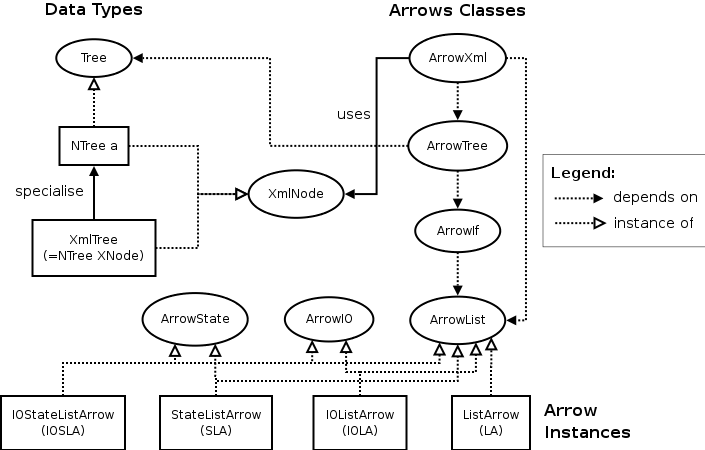
\includegraphics[width=\textwidth]{images/hxt-structure.eps}
\end{figure}

%------------Chapter Three -----------------------
\chapter{Example RDF/XML Processing}
\section{Introduction}
Now that the structure, the basic ideas as well as the different classes of the Haskell XML Toolbox have been described, this chapter will demonstrate how to design a program with it. The implementation of an RDF/XML parser was chosen as an example, because all parts of the Haskell XML Toolbox, from simple file handling to complex arrows, are needed for reaching this goal. But before starting the programming, the language and the idea of RDF need to be discussed.\\
The Resource Description Framework (RDF) is a language for representing information about resources in the World Wide Web \cite{RDF:Primer}. The main intention of RDF is to represent meta data about Web resources, e.g. the author, title, or the modification date of the Web page. However, RDF can also be used more generally to represent information about all kinds of things that can be identified on the Web. This can be information about the goods of an online shop or the description of a Web service provided by a Web page. \\
The idea of RDF is not to provide another concept of displaying information to people like the Hypertext Markup Language (HTML), but rather to make the information processable by applications. The handling of RDF is based on a common framework, so the information can be processed outside the environment in which it was created or even combined with other information.\\
In RDF, every resource can be identified by Web identifiers called Uniform Resource identifiers (URI). The resources are described in terms of simple properties and property values. This defines a simple but flexible data model which represents the resources as graphs of nodes and arcs.\\  
The following sections give an overview of the  concept of RDF based on the following three documents: Primer \cite{RDF:Primer}, concepts \cite{RDF:Concepts} and syntax specification \cite{RDF:Syntax}.

\subsection{Basic Concepts of RDF}
The purpose of RDF is to describe resources in the Web. In other words, it is used to make statements about resources. As already mentioned, these statements are defined as a thing identified by an URI and described in terms of a property with a value. In an RDF statement, these three things are named \textit{subject}, \textit{predicate} and \textit{object}. Together they form a pattern which is called a {\it triple}. Like in natural languages, the subject is the thing which is described and identified, the predicate is the property of the subject and the object is the value of the predicate. An example of an English statement is:
\\[1ex]
{\bf http://www.example.org/index.html} has a {\bf creator} whose value is {\bf John Smith}
\\[1ex]
The RDF terms of this statement are:
\begin{itemize}
  \item the {\it subject} is the Uniform Resource Locater (URL) to identify the Web page http://www.example.org/index.html
  \item the {\it predicate} is the word ``creator''
  \item the {\it object} is the phrase ``John Smith''
\end{itemize}
This example shows how RDF is structured, but it is not complete. In RDF, everything is identifiable and ambiguity should be avoided to ensure that the statements are machine-processable. Ambiguity among subjects, predicates or objects would mean that they cannot be clearly identified and, therefore, not processed by an application. To solve this problem, RDF uses Uniform Resource Identifier (URI) \cite{URIS} extended with references called URI reference or {\it URIref}.\\
In the example above, the subject, namely the Web page, is identified by an URL. But in order to identify every part of the statement, it is also necessary to describe aspects which have no network locations and URLs. URIs are more general and not limited to identifying things in the Web. URLs are, in fact, only a particular kind of URI.\\
\\
To be machine-processable, RDF needs to be represented in a way that applications can read it. There are different languages to serialise RDF. One is {\it N-Triples}, which is often used to explain RDF and to write down simple statements because it is very short and clear. The other one is {\it RDF/XML}, the official language, recommended by the W3C. RDF/XML uses the Extensible Markup Language (XML), which allows to design own document formats and write documents in that format. A detailed description about XML can be found in the document \cite{XML}. RDF/XML and its syntax will be described more thoroughly in section \ref{rdfsyntax}.
\subsection{Model of RDF}\label{rdfmodel}
The example statement of the last section:
\\[1ex]
{\bf http://www.example.org/index.html} has a {\bf creator} whose value is {\bf John Smith}
\\[1ex]
can also be represented by the following triple:
\begin{itemize}
  \item the subject: \texttt{http://www.example.org/index.html}
  \item the predicate: \texttt{http://purl.org/dc/elements/1.1/creator}
  \item the object: \texttt{http://www.example.org/staffid/87540} 
\end{itemize}
In RDF, neither the subject nor the predicate must be character strings. That is because every element of a triple should be identifiable and only the object can be a so-called \textit{literal}. Those literals can be \textit{plain literals}, which is a simple character string, or \textit{typed literals}, where the literal has an additional data type information. Both, plain and typed literals, can contain Unicode characters that allow to represent information from many languages directly.\\
The URIrefs used in triples are often organised so that they define a vocabulary. The predicate URIref \texttt{http://purl.org/dc/elements/1.1/creator}, for example, is part of the Dublin Core vocabulary \cite{DC}. In this vocabulary there are definied several commonly used terms, like the term \textit{creator}. The advantage of vocabularies lies in their reusability. Applications using the same vocabulary understand or interpret the predicates of triples in the same way, since their meaning and their usage are defined. Vocabularies for RDF are written in the RDF Vocabulary Description Language \cite{RDF:Schema}, which shall not be described here.\\
The statements of RDF can be modelled as nodes and arcs in a graph and in this notation a statement is represented by
\begin{itemize}
    \item a node for the subject
    \item a node for the object
    \item a directed arc from the subject node to the object node for the predicate
\end{itemize}
So, the statement above can be modelled by the graph in figure \ref{graph1}.
\begin{figure}[H]
        \caption{Simple RDF Graph}
        \label{graph1}
        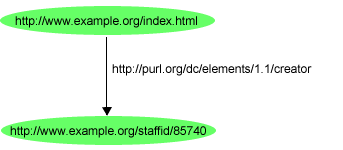
\includegraphics[width=0.7\textwidth]{images/simplegraph1.eps}
\end{figure}
Another way to represent or serialise RDF statements using English statements is the \textit{N-Triples} notation, which is a fixed subset of N3 \cite{N3}. The N-Triples notation requires that URI references are written out completely in angle brackets. This can result in very long lines per page. Therefore, in order to abbreviate full URI references, qualified names (see section \ref{xmltree}) are used to avoid this. The following list includes the qualified names that are used throughout this document and without explicitly specifying them each time:
\begin{itemize}
\item prefix \texttt{rdf:} namespace URI: \texttt{http://www.w3.org/1999/02/22-rdf-syntax-ns\#}
\item prefix \texttt{dc:} namespace URI: \texttt{http://purl.org/dc/elements/1.1/}
\item prefix \texttt{ex:} namespace URI: \texttt{http://www.example.org/}
\item prefix \texttt{exterms:} namespace URI: \texttt{http://www.example.org/terms/}
\item prefix \texttt{exstaff:} namespace URI: \texttt{http://www.example.org/staffid/}
\item prefix \texttt{xsd:} namespace URI: \texttt{http://www.w3.org/2001/XMLSchema\#}
\end{itemize}
The next listing shows a group of statements with additional information added to the example above in N-Triples notation and using this new shorthand: 
\begin{blank}[caption=Group of Statements with N-Triple Notation]
ex:index.html   dc:language             "en" .
ex:index.html   exterms:creation-date   "August 16, 1999" .
ex:index.html   dc:creator              exstaff:85740 .
\end{blank} 
The RDF graph of that group is shown in figure \ref{graph2}.
\begin{figure}[H]
        \caption{Compound RDF Graph}
        \label{graph2}
        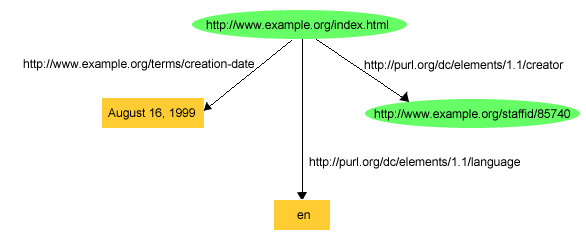
\includegraphics[width=\textwidth]{images/simplegraph2.eps}
\end{figure}
This example illustrates the use of vocabularies: An organisation such as example.org has a vocabulary consisting of URIrefs starting with the prefix \texttt{http://www.ex\-ample.org/\ terms/} for terms it uses in its business, such as ``creation-date'' or ``product''. Another vocabulary of the organisation is to identify its employees with URIrefs starting with \texttt{http://\-www.ex\-ample.org/staffid/}. RDF itself uses the same approach to define its own vocabulary of terms with special meanings in RDF. As shown in the list above, the URIrefs in the RDF vocabulary all begin with \texttt{http://www.w3.org/\ 1999/02/22-rdf-syntax-ns\#}, which is conventionally associated with the QName prefix \texttt{rdf:}.\\
In addition to this, it is crucial to distinguish between any meaning that RDF for itself associates with terms such as \texttt{dc:creator} and externally-defined meaning that programs might associate with those terms. Only the semantics of the RDF vocabulary and the graph syntax are directly defined in the documents \cite{RDF:Syntax} and RDF-Semantics \cite{RDF:Semantics}. The meaning of any other vocabularies is defined somewhere externally to RDF. Thus, generic RDF applications like parsers, would only recognise a statement with a specific vocabulary as a valid triple, but would not add and verify any special meaning that might be associated with any terms of the vocabulary.

\subsubsection{Blank Nodes}\label{blanknodes}
Graphs may also include nodes without URIrefs, i.e. \textit{blank nodes}. The idea behind blank nodes is to represent something that does not have an URIref, but can be described in terms of other information. As an example, figure \ref{graph3} shows a graph which represents the statement ``the document 'http://www.w3.org/TR/rdf-syntax-grammar' has a title 'RDF/XML Syntax Specification (Revised)' and has an editor, the editor has a name 'Dave Beckett' and a home page 'http://purl.org/net/dajobe' ''.
\begin{figure}[H]
        \caption{Graph with a Blank Node}
        \label{graph3}
        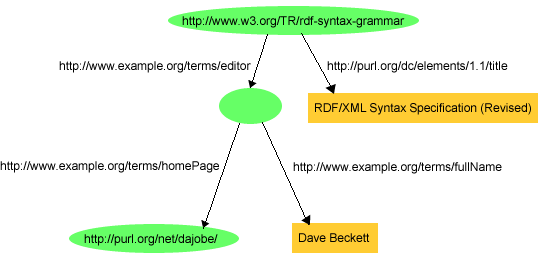
\includegraphics[width=\textwidth]{images/blankNode.eps}
\end{figure}

The concept of the editor of a Web page does not need to be referred directly from outside a particular graph and hence, does not require a ``universal'' identifier. The blank node simply provides the necessary connectivity between the remaining parts of the graph. However, to represent this graph with the N-Triples notation, the blank nodes also need some form of explicit identifier. N-Triples use \textit{blank node identifiers} having the form \texttt{\_:name} for that, where \texttt{name} can be any kind of character string. In most cases, this is a number. For instance, a blank node identifier \texttt{\_:id1} might be used to refer to the blank node. To keep this example short, only the subgraph with the blank node is shown:
\begin{blank}[caption=Triples with Blank Nodes]
<http://www.w3.org/TR/rdf-syntax-grammar>   exterms:editor   _:id1 .

_:id1   exterms:homePage    <http://purl.org/net/dajobe> .

_:id1   exterms:fullName    "Dave Beckett" .
\end{blank} 
Blank node identifiers are not actual parts of the RDF graph, like URIrefs and literals are. They serve as representatives of the blank nodes in a graph and distinguish one blank node from another when the graph is written in the N-Triple form. Additionally, blank node identifiers also have significance only within the triples representing a \textit{single} graph.\\
Because RDF can only represent \textit{binary} relations directly, blank nodes also provide a way of dealing with n-ary relations by breaking them up into a group of separate binary relations.

\subsubsection{Typed Literals}
In some situations, it might be more appropriate to store some kind of type information to the plain literal of a statement. For example, if the age of a person is to be recorded, it does not make sense to use a plain literal for this, like illustrated in the next listing:
\begin{blank}
exstaff:85740   exterms:age     "27" .
\end{blank}
An application processing this statement cannot ``know'' that the literal ``27'' is a decimal number and not a character string. Therefore, the data type information of this literal is added to the statement like it is done in database systems or programming languages. In RDF, these extended literals are called \textit{type literals}. The example above can be rewritten using a typed literal to store the age:
\begin{blank}
exstaff:85740   exterms:age     "27"^^xsd:integer .
\end{blank}
The same example is show as a graph in figure \ref{typedLiteral}.
\begin{figure}[H]
        \caption{Graph with a Typed Literal}
        \label{typedLiteral}
        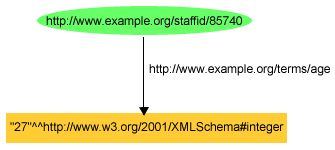
\includegraphics[width=0.7\textwidth]{images/typedLiteral.eps}
\end{figure}
In this example the data type \texttt{integer} defined in the XML Schema \cite{XML:Schema} data types is used. It is very important to keep in mind that the data types of the typed literals are not validated by generic RDF applications. As it is the case with the vocabulary, the data type definition is done externally from the RDF definition, which means that an RDF parser cannot determine whether a literal is valid or not. This has to be done by the applications which know how to process these particular data types.\\ \\
This section has presented an introduction to the concepts of RDF. It has shown how RDF can be used to store all kinds of data and that RDF graphs are similar to the way of recording information in simple relational databases.

\subsection{RDF/XML - Syntax}\label{rdfsyntax}
Although the conceptual model of RDF is a graph, it is also necessary to write down and exchange or, in other words, to serialise RDF graphs. The N-Triples notation, which has been already introduced, can be used for this but it was only intended as a shorthand notation. RDF/XML instead, is the normative syntax for serialising RDF graphs and is defined in the RDF/XML Syntax Specification \cite{RDF:Syntax}. The basic ideas behind the RDF/XML syntax can be illustrated by using some of the examples presented previously. The example in listing \ref{statementwplain} has taken the first example and has replaced the URIref of the object by a plain literal.
\begin{blank}[caption=RDF Statement with Plain Literal,label={statementwplain}]
ex:index.html   exterms:creator     "John Smith"
\end{blank}
This RDF statement can be encoded in RDF/XML Syntax as the following listing:
\begin{xmlnb}[caption={RDF/XML for the Creator Concept},label={rdfxml1}]
<?xml version="1.0"?>
<rdf:RDF xmlns:rdf="http://www.w3.org/1999/02/22-rdf-syntax-ns#"
            xmlns:exterms="http://www.example.org/terms/">
    
    <rdf:Description rdf:about="http://www.example.org/index.html">
        <exterms:creator>John Smith</exterms:creator>
    </rdf:Description>

</rdf:RDF>
\end{xmlnb}
Lines 1-3 are the ``introduction'' of the RDF/XML document. First, in line one, there is the XML declaration to indicate that the following content is XML. Then, in line two and three, there begins an \texttt{rdf:RDF} element which indicates that the following content up to the end tag is RDF. The namespace declarations for the RDF namespace, defining the terms from the RDF vocabulary and all the others which are used throughout this document, are also written down in these lines. Although the RDF namespace and the \texttt{rdf:RDF} element are optional in situations where the XML can be identified as an RDF/XML document by context, it is always better to provide them, since this makes the documents much clearer.\\
In line five there is the \texttt{rdf:Description} element, which indicates the start of a \textit{description} of a resource and is also called \textit{node element}. What this statement is \textit{about}, is specified in the \texttt{rdf:about} attribute. The content of this attribute is the URIref of the subject. The following line, line six, provides a \textit{property element}, which represents the predicate and object of the statement. The qualified name \texttt{exterms:creator} of this element specifies the predicate and the content of the property element is the plain literal \texttt{John Smith}, which is the object.\\
The listing \ref{rdfxml1} illustrates the basic ideas of RDF/XML. There are several other ways of representing an RDF statement in XML and also a lot of abbreviations to keep the RDF/XML documents from becoming too big. All of these options are described in \cite{RDF:Syntax} and this section introduces only those which are shown in \\\cite{RDF:Primer}.
\\
Making more than one statement about the same resource can be represented in RDF/XML by using the lines 5-7 in listing \ref{rdfxml1} for every new statement. To avoid this overhead of repeating the same \texttt{rdf:Description} element for every statement, RDF/XML allows multiple property elements, representing the predicates and objects for the same subject resource. For example, listing \ref{rdfxml2} represents the following group of statements:
\begin{blank}
ex:index.html   dc:creator              exstaff:85740
ex:index.html   exterms:creation-date   "August 16, 1999"
ex:index.html   dc:language             "en"
\end{blank}
These triples are the same as the RDF graph shown in figure \ref{graph2}.
\begin{xmlnb}[caption={Multiple Properties},label={rdfxml2}]
<?xml version="1.0"?>
<rdf:RDF xmlns:rdf="http://www.w3.org/1999/02/22-rdf-syntax-ns#"
            xmlns:dc="http://purl.org/dc/elements/1.1/"
            xmlns:exterms="http://www.example.org/terms/">
    
  <rdf:Description rdf:about="http://www.example.org/index.html">
    <exterms:creation-date>August 16, 1999</exterms:creation-date>
    <dc:language>en</dc:language>
    <dc:creator rdf:resource="http://www.example.org/staffid/85740"/>
  </rdf:Description>

</rdf:RDF>
\end{xmlnb}
Apart from showing how to use multiple property elements, the listing \ref{rdfxml2} also introduces a new form of property element. Unlike the first two properties, the property in line nine is an empty element with an \texttt{rdf:resource} attribute. This attribute represents a property whose value is another \textit{resource}, rather than a literal. If the URIref of this resource has been written in the same way as the literal values, the URIref would not be a resource identifier but a character string. Unfortunately, the URIref cannot be abbreviated as a qualified name and has to be written out, since it is being used as an attribute value.\\
Using blank nodes to describe resources is another technique of RDF. Blank nodes are nodes which do not have an URIref but can be described in terms of other information as discussed in section \ref{blanknodes}. RDF/XML provides several ways to represent graphs containing those nodes, but only the most direct approach should be illustrated here. This is to assign a \textit{blank node identifier} to each blank node. A blank node identifier only identifies a blank node within a particular RDF/XML document and is, in contrast to an URIref, unknown outside the document. In order to refer to a blank node in RDF/XML, the \texttt{rdf:nodeID} attribute and the identifier as its value are used. This attribute can appear in places where the URIref of a resource would otherwise be and replaces the \texttt{rdf:about} attribute of node elements (elements with the name \texttt{rdf:Description}). The example in listing \ref{rdfxml3} shows the RDF/XML corresponding to figure \ref{graph3}.
\begin{xmlnb}[caption={Blank Nodes in RDF/XML},label={rdfxml3}]
<?xml version="1.0"?>
<rdf:RDF xmlns:rdf="http://www.w3.org/1999/02/22-rdf-syntax-ns#"
            xmlns:dc="http://purl.org/dc/elements/1.1/"
            xmlns:exterms="http://www.example.org/terms/">

  <rdf:Description rdf:about="http://www.w3.org/TR/rdf-syntax-grammar">
    <dc:title>RDF/XML Syntax Specification (Revised)</dc:title>
    <exterms:editor rdf:nodeID="abc"/>
  </rdf:Description>

  <rdf:Description rdf:nodeID="abc">
    <exterms:fullName>Dave Beckett</exterms:fullName>
    <exterms:homePage rdf:resource="http://purl.org/net/dajobe/"/>
  </rdf:Description>

</rdf:RDF>
\end{xmlnb}
In listing \ref{rdfxml3} the value of the \texttt{exterms:editor} property is a blank node with the identifier \texttt{abc}. The blank node itself is defined in line 11 as the subject of two statements.\\
\\
Instead of using  plain literals as usual, the typed literals introduced in section \ref{rdfmodel} may be used as well. This can be done in RDF/XML by adding an \texttt{rdf:datatype} attribute with the data type URIref as its value to the property element. The following listing illustrates the graph shown in figure \ref{typedLiteral} in the RDF/XML syntax:
\begin{xmlnb}[caption={Typed Literal in RDF/XML},label={rdfxml4}]
<?xml version="1.0"?>
<rdf:RDF xmlns:rdf="http://www.w3.org/1999/02/22-rdf-syntax-ns#"
            xmlns:exterms="http://www.example.org/terms/">

  <rdf:Description rdf:about="http://www.example.org/staffid/85740">
    <exterms:age rdf:datatype=
      "http://www.w3.org/2001/XMLSchema#integer">27
    </exterms:age>
  </rdf:Description>

</rdf:RDF>
\end{xmlnb}

The RDF/XML Syntax described so far provides a simple but general way of expressing RDF graphs. This simple approach gives the most direct representation of the actual graph structure. Some other additional abbreviations provided by RDF/XML will be introduced in section \ref{rdfparser} along with the example RDF/XML parser. 

\subsection{SPARQL -- Query Language for RDF} \label{sparql}
The approach of storing information in RDF is very similar to that of simple relational databases. Almost every relational database provides the Structured Query Language (SQL) to access the information recorded in the tables of a database. SQL provides several commands to manipulate and to search for data. It seems likely to provide such a data access language also for RDF, which could be used to query the information stored in RDF graphs. There are several approaches of query languages for RDF and one of them should be introduced here. This is the query language part of the \textit{Protocol and RDF Query Language} (SPARQL) \cite{SPARQL} which is still under development and not finished yet. SPARQL provides a lot of features to search for information in RDF, like querying more than one graph and connecting several RDF stores. As this document intends to exemplify how to implement an RDF/XML parser with a small query engine, only the basic language features of SPARQL should be introduced here.\\
The idea of the SPARQL query language is based on matching \textit{graph patterns}. There are several versions of graph patterns. The simplest one is the \textit{triple pattern} which is the same as an RDF triple but with the possibility of a variable in any of the subject, predicate or object positions. An exact match of this triple pattern to an RDF graph is needed to fulfill a pattern. A simple query which searches for the title of a book in the following data:
\begin{blank}
ex:book/book1 dc:title "SPARQL Query"
\end{blank}
shows the next listing:
\begin{blank}[caption=Simple SPARQL Query]
SELECT ?title
WHERE { <http://www.example.org/book/book1> 
        <http://purl.org/dc/elements/1.1/title> 
        ?title . }
\end{blank}
The result of this query would be:\\ \\
\begin{tabular}[c]{|c|}\hline
{\sf\bf title} \\ \hline
{\tt "SPARQL Query"}\\ \hline
\end{tabular}\\ \\
A query always consists of two parts, the \texttt{SELECT} clause and the \texttt{WHERE} clause. The \texttt{SELECT} clause specifies the variables, which should be returned by the query. The \texttt{WHERE} clause contains the graph pattern. In this case the graph pattern consists one single triple pattern. Graph patterns can also be of other pattern types. Every pattern adds additional functionality to SPARQL. These additional pattern types will not be taken into consideration.\\
The triple pattern consists of three query terms. These can be an URIref delimited by ``$<$$>$''. The object can also be a literal which is delimited by single or double quotes and can be followed by an optional language tag, introduced with '@', or an optional data type URI, introduced by \lstinline!'^^'!. As a convenience, integers, floating point numbers and boolean values can be directly written and are interpreted as typed literals of data type \texttt{xsd:integer}, \texttt{xsd:double} or \texttt{xsd:boolean}.\\
The variables used in a SPARQL query have a global scope and are indicated by '?' or '\$'.\\
The term ``binding'' is used as a descriptive term to refer to a pair of variable and RDF term. These bindings result in tabular form so if variable x is bound to ``Fred'' it is shown as:\\ \\
\begin{tabular}[c]{|c|}\hline
{\sf\bf x} \\ \hline
{\tt "Fred"}\\ \hline
\end{tabular}\\ \\
The results of a query can also be returned in RDF, in a special XML format defined in \cite{SPARQL:Result} or in forms specific to the implementation.\\
The matching of a graph pattern to a graph, gives bindings between the variables of the triple patterns and the RDF terms. This means, the triple pattern, with the variables replaced by the corresponding RDF terms, is a triple of the graph being matched. This process is also called \textit{substitution}.\\
The last example has shown how to search for only one triple. In the following example, the data consists of two triples with blank nodes as the subject and the query also consists of two triple patterns. This graph pattern only matches if \textit{each} of the triple patterns matches with the \textit{same} substitution. The data is:
\begin{blank}
_:a dc:name "Johnny" .
_:a dc:mbox <mailto:jlow@example.com> .
\end{blank}
The query to search for the mail address is:
\begin{blank}
SELECT ?mbox
WHERE { ?x <http://purl.org/dc/elements/1.1/name> "Johnny" .
        ?x <http://purl.org/dc/elements/1.1/mbox> ?mbox }
\end{blank}
This leads to the following result:\\ \\
\begin{tabular}[c]{|c|}\hline
{\sf\bf mbox} \\ \hline
{\tt <mailto:jlow@example.com>}\\ \hline
\end{tabular}\\ \\
With SPARQL, it is also possible to deal with multiple matches. The example above could have two mail addresses as a result if the data contained two entries with the name ``Johnny''.\\
Triple patterns are written as a list of subject, predicate and object, which can result in very long lists and can therefore be abbreviated. The \textit{predicate-object list} allows to write down the subject only once where several triple patterns with the same subject are needed. The predicate-object list is then delimited by a ';' like shown in the next listing:
\begin{blank} 
?x  dc:creator          ?name ;
    dc:creation-date     ?date .
\end{blank}
Another way of abbreviating triple patterns are \textit{object lists}, which can be used when triple patterns share both subject and predicate. The following listing illustrates how the object list is used.
\begin{blank} 
?x  dc:creator  "Alice" , "Alice_" .
\end{blank}
This is the same as writing the triple patterns in the following form:
\begin{blank} 
?x  dc:creator  "Alice" .
?x  dc:creator  "Alice_" .
\end{blank}

Like section \ref{rdfsyntax}, this section illustrated some, but not all of the abbreviations and language features of the SPARQL query language. A number of additional ones will be described in further detail in the next sections, but the language shown so far already provides enough features to write simple and useful queries for RDF triples.
  
\section{Writing the RDF/XML Parser} \label{rdfparser}
\subsection{Introduction}
The RDF/XML parser, which shall now be implemented, is structured and based on the complexity of the tasks. First of all, a function or module is needed which takes care of the I/O handling, i.e. reading an RDF document and presenting the result of the parsing process. Then, the real processing of the document needs to be implemented, which is also separated in several parts. The first part is to normalise all the RDF/XML abbreviations into a simple and normative RDF/XML document. This normalised document is then processed and the result is stored in a new data structure. After that, the data structure can be printed out in several formats like the N-Triples notation or a simple RDF/XML representation. Furthermore, a SPARQL parser and a module for searching in the RDF data structure is also a part of it, in order to provide simple query features.

\subsection{Main Function and Option Handling}
The first part of a program is the main function, which is the ``main entry point''. The file handling and the additional processing of the XML document are coordinated in this function.    
The Haskell XML Toolbox provides -- besides the arrows introduced in section \ref{mainarrows} -- the module \texttt{XmlStateFilterInterface}, which consists of compound arrows for reading, parsing, validating and writing XML documents. The most important arrows of this module are \texttt{readDocument} and \texttt{writeDocument}. The arrow \texttt{readDocument} is the main document input arrow. It can be configured by an option list of type \texttt{Attributes} and takes the file name of the document which should be read as parameter. The attribute list of \texttt{readDocument} is stored in the global state component to ensure that it can be accessed everywhere in the program. Some of the available options are:
\begin{itemize}
  \item \texttt{a\_validate} : validate document, else skip validation (default)
  \item \texttt{a\_check\_namespaces} : check namespaces, else skip namespace processing (default)
  \item \texttt{a\_canonicalize} : canonicalise document (default), else skip canonicalisation
  \item \texttt{a\_remove\_whitespace} : remove all whitespace, used for document indentation, else skip this step (default)
  \item \texttt{a\_trace} : trace level: values: 0 - 4
\end{itemize}
The writing of XML documents to files is done by the arrow \texttt{writeDocument}. Like \texttt{readDocument}, it takes a list of options and the file name of the document which should be written. The full list of the available options for both arrows is listed in appendix \ref{options}.\\
The next listing, for example, illustrates how to write a main function that reads an RDF file ``simple.rdf'' in, processes all namespaces, removes all white spaces and then creates a new RDF file ``output.rdf'' out of it:
\begin{code}[caption=First Main Function]
main :: IO ()
main
  = do
    runX ( readDocument [(a_check_namespaces,"1"),
                         (a_remove_whitespace,"1")] 
                        "simple.rdf"
           >>>
           writeDocument [] "output.rdf"
         )
    return ()
\end{code}
Unlike the two options handed over to \texttt{readDocument}, the arrows \texttt{removeAllWhiteSpace} and \texttt{propagateNamespaces} can be used to delete the whitespaces and process all namespaces. Line-breaks to indent a XML document are interpreted as XML text nodes. When processing those documents, it is crucial to call \texttt{removeAllWhiteSpace}, since these extra text nodes are also returned by \texttt{getChildren}. Sometimes, the number of chil-nodes of an element are of interest and text nodes containing line-breaks disturb or cover up the real number which maybe leads to incorrect results.\\
The function \texttt{runX}, described in section \ref{xmlstate}, is used to run the processing. In this case, it consists of the two arrows  \texttt{readDocument} and \texttt{writeDocument} combined with the operator {\tt ($>$$>$$>$)}, which results in an I/O action. This action is executed by \texttt{runX} and the main function ends by returning the empty tuple. Several errors, like XML syntax error, can occur during the processing. These errors, however, are ignored and the main function always ends successfully.\\
To enable the error handling in the example above, the arrow \texttt{getErrStatus} from the module \texttt{XmlIOStateArrow} reads the error status from the global state, which can then be used to determine, how the main function should end. The example in listing \ref{mainerr} shows how the main function can be rewritten, so as to enable error handling and tracing parse errors while processing.
\begin{code}[caption=Main Function with Error Handling,label=mainerr]
main
  = do
    [rc] <- runX ( readDocument [(a_trace,"1")] 
                                "simple.rdf"
                   >>>
                   removeAllWhiteSpace >>> propagateNamespaces
                   >>>
                   writeDocument [] "output.rdf"
                   >>>
                   getErrStatus
                 )
    exitWith ( if rc >= c_err
               then ExitFailure (-1)
               else ExitSuccess )
\end{code}
When including the main function from the example above into a Haskell module, two modules have to be imported. One of them is the module \texttt{Text.XML.HXT.Arrow} which is the application programming interface to the arrow modules of the Haskell XML Toolbox and exports all important arrows, basic data types and functions. The other one is the module \texttt{System.Exit} from the standard Haskell libraries which is used to get the functions for advanced program termination.\\
However, the example above is still not completed. Another considerable feature which should be provided by every program is to deal with command-line options. Furthermore, the name of the input and output file should not be hard coded but rather specified by a command-line argument. Therefore, the main function has to be rewritten again.
\clearpage
\begin{code}[caption=Main Function with Commandline Options,label=maincmd]
main
    = do
      argv      <- getArgs         
      (al, src) <- cmdlineOpts argv       
      [rc]      <- runX (processDocument al src)
      exitWith ( if rc >= c_err
                 then ExitFailure (-1)
                 else ExitSuccess )
\end{code}
Listing \ref{maincmd} shows that, the command-line parameters are collected first by the Haskell function \texttt{getArgs}. After that, the function \texttt{cmdlineOpts} processes these parameters and returns a pair of the list of processed arguments and the input file name. This pair, then, is handed over to the arrow \texttt{processDocument} which is executed by \texttt{runX}. Finally, the error handling is done in the same way as shown in the last example.\\
The function \texttt{cmdlineOpts} parses the command-line parameters, prints the list of available command-line arguments or terminates the program if no input file name has been specified. The definition of it shall not be described here in detail, because it is not a Haskell XML Toolbox specific function, but a standard Haskell code.\\
The main function is much shorter now that the processing arrows are encapsulated by the arrow \texttt{processDocument}, which is defined as follows:
\begin{code}[caption=processDocument, label=processdocument]
processDocument :: Attributes -> String -> IOSArrow b Int
processDocument al qr src
    = readDocument al src 
      >>>
      removeAllWhiteSpace >>> propagateNamespaces
      >>>
      writeDocument al (fromMaybe "" (lookup a_output_file al))
      >>>
      getErrStatus
\end{code}
The arrow takes the attributes and the name of the input file as extra parameters. These arguments are handed over to \texttt{readDocument}. Moreover, the command-line option for the name of the output file is looked up in the list of parameters \texttt{al}. If this parameter does not exist, the output is printed to the standard output. This list can contain any options, allowed by \texttt{readDocument} and \texttt{writeDocument}. Later in this section, an extra command-line option will be added to the available list of arguments.\\
The program described so far is already a fully working application, which parses a XML document and writes it back to a file or the standard output. However, it does not contain any RDF/XML specific arrows yet. The arrow \texttt{processDocument} can be extended easily by any arrow which processed XML somehow. In the next section this will be shown by implementing parser arrows for RDF/XML.

\subsection{Parsing RDF/XML}
Before starting to parse the full RDF/XML syntax, only a subset of it is processed. This subset covers all the features described in section \ref{rdfsyntax}. The additional syntax abbreviations and their processing are discussed in the next section.

\subsubsection{Simple Processing Arrows}
The first simple RDF/XML document which should be processed by the parser is the document presented in listing \ref{rdfxml1}. The next listing shows this RDF document in order to recall the syntax of RDF/XML (the XML and namespace declaration have been removed):
\begin{blank}
<rdf:Description rdf:about="http://www.example.org/index.html">
    <exterms:creator>John Smith</exterms:creator>
</rdf:Description>
\end{blank}
It contains no abbreviations and has only one RDF triple with a plain literal as the object. First of all, the processing functions return their results in a simple XML document and later it will be shown how to store these results in a special data structure for RDF. The structure of this XML document is illustrated in the next listing, using the data of listing \ref{rdfxml1}:
\begin{blank}[caption=Simple Triple Representation,label=output]
<triple>
    <subject>http://www.example.org/index.html</subject>
    <predicate>http://www.example.org/terms/creator</predicate>
    <object>John Smith</object>
</triple>
\end{blank}
To achieve this result, every \texttt{rdf:Description}-element has to be selected by processing the whole XML document tree. The following listing shows the predicate, which tests whether an element has the name \texttt{rdf:Description} and the attribute \texttt{rdf:about}.
\begin{code}[caption={Predicate detecting Node Elements}] 
isNodeElem :: (ArrowXml a) => a XmlTree XmlTree
isDesc
  = isElem >>> hasQName rdf_Description >>> hasQAttr rdf_about
\end{code}
The constants \texttt{rdf\_Description} and \texttt{rdf\_about} are of type \texttt{QName} and represent the qualified names.\\
This predicate can now be applied to the whole document tree. If the predicate holds, this element can be further processed. The traversing through the tree is done by the arrow \texttt{deep}: 
\begin{code}[caption={Apply the Predicate to the Tree}] 
processRDF :: (ArrowXml a) => a XmlTree XmlTree
processRDF 
  =  processChildren (deep (isNodeElem `guards` getTriple))
\end{code}
The arrow \texttt{getTriple} does the actual processing of the \texttt{rdf:Description} elements. It selects the value of the \texttt{rdf:about} attribute and creates an element with the name ``subject'' and the value as a text element. The same is done with the property element by selecting the predicate and object value and generating elements with the name ``predicate'' and ``object'' out of it. These three elements are then added to the list of children of an element called ``triple'':
\begin{code}[caption={getTriple}]
getTriple :: (ArrowXml a) => a XmlTree XmlTree
getTriple 
  = selem "triple"
    [getQAttrValue rdf_about >>> selem "subject" [mkText]
    ,getChildren >>> getUniversalUri 
                 >>> selem "predicate" [mkText]
    ,selem "object" [getChildren>>>getChildren]
    ]
\end{code} 
The arrow \texttt{processRDF} can now be added to the \texttt{processDocument} arrow from listing \ref{processdocument}, so that it processes the XML tree generated by \texttt{readDocument} and passes the result of it to the arrow \texttt{writeDocument}.\\
The resulting program is already able to process very simple RDF documents with one or more triples, but every triple has to be declared explicitly and no abbreviations are allowed. In order to process the multiple property elements as shown in listing \ref{rdfxml2}, the function above has to be rewritten, because the URIref of the subject is needed several times. The function \texttt{getTriple} now takes an additional parameter of type string which is the URIref of the subject to ensure that it can be used more than once. The listing \ref{getTriple} presents the rewritten function \texttt{getTriple}.
\begin{code}[caption={getTriple for Multiple Properties},label=getTriple]
getTriple subject
  = getChildren >>> selem "triple"
    [selem "subject" [txt subject]
    , getUniversalUri >>> selem "predicate" [mkText]
    , selem "object" [getChildren]
    ]
\end{code}
Furthermore, a new arrow is needed to select the value of the \texttt{rdf:about} attribute. This new arrow is called processSubject and is defined as follows:
\begin{code}
processSubject :: (ArrowXml a) => a XmlTree XmlTree
processSubject = arr getTriple $< getQAttrValue rdf_about
\end{code}
It hands the value of the attribute over to the arrow \texttt{getTriple} via the combinator \texttt{\$<}, which allows the programmer to use a parameter more than once (see section \ref{arrowlist}). This arrow shows, that the special combinators for point-wise programming are highly practical. Without them the code of such a simple arrow would be awkward and confusing.\\
Now, \texttt{processSubject} and not \texttt{getTriple} has to be applied to the whole tree in the arrow \texttt{processDocument}. Every time the predicate \texttt{isNodeElem} holds, the \texttt{rdf:about} value is selected and handed over to \texttt{getTriple}, which generates a triple element for every child-node of the \texttt{rdf:Description} element.\\
\\
The next RDF/XML syntax feature that should be supported by the parser are blank nodes. There are several ways of representing blank nodes in RDF/XML, but first only blank nodes with a explicit blank node identifier should be processed. Therefore, the predicate \texttt{isNodeElem} has to be rewritten, because an \texttt{rdf:Description} element can also have a \texttt{rdf:nodeID} attribute carrying the blank node identifier instead of the \texttt{rdf:about} attribute. The choice between these two possibilities is made by the combinator \texttt{orElse}, as the next listing shows:
\enlargethispage{1cm}
\begin{code}[caption=isNodeElem with Blank Node Test, label=isNodeElem]
isNodeElem = isElem >>> hasQName rdf_Description 
         >>> (hasQAttr rdf_nodeID `orElse` hasQAttr rdf_about)
\end{code}

In addition to \texttt{isNodeElem}, the arrow \texttt{processSubject} also has to be rewritten, since the blank node identifier has to be selected as well as the URIref. The following listing illustrates how the choice between attributes can be made by the \texttt{choiceA}-construction (the type signature has been removed):
\begin{code}[caption=processSubject with Blank Node]
processSubject 
  = arr getTriple 
    $< choiceA [hasQAttr rdf_about :-> getQAttrValue rdf_about
               ,hasQAttr rdf_nodeID:-> getQAttrValue rdf_nodeID
               ]
\end{code}
Moreover, the processing of the object of a triple has to be changed, since an object can also have an \texttt{rdf:nodeID} attribute referring to a blank node or an \texttt{rdf:resource} with an URIref. This is done by the arrow \texttt{processObject} which also uses \texttt{choiceA} to deal with the different cases:
\begin{code}
processObject :: (ArrowXml a) => a XmlTree XmlTree
processObject
  = choiceA [isResource     :-> getQAttrValue rdf_resource 
            ,isBlankNodeRef :-> getQAttrValue rdf_nodeID
            ,this           :-> getChildren >>> getText 
            ]
    >>>
    selem "object" [mkText]
\end{code}
The predicates \texttt{isResource} and \texttt{isBlankNodeRef} test if the element is empty and has the right attribute. Now, the creation of the ``object'' element can be replaced in \texttt{getTriple} by \texttt{processObject} and the application is able to process RDF documents with blank nodes like the one in listing \ref{rdfxml3}, which would generate the following output:
\begin{blank}
<triple>
  <subject>http://www.w3.org/TR/rdf-syntax-grammar</subject>
  <predicate>http://purl.org/dc/elements/1.1/title</predicate>
  <object>RDF/XML Syntax Specification (Revised)</object>
</triple>
<triple>
  <subject>http://www.w3.org/TR/rdf-syntax-grammar</subject>
  <predicate>http://www.example.org/terms/editor</predicate>
  <object>abc</object>
</triple>
<triple>
  <subject>abc</subject>
  <predicate>http://www.example.org/terms/fullName</predicate>
  <object>Dave Beckett</object>
</triple>
<triple>
  <subject>abc</subject>
  <predicate>http://www.example.org/terms/homePage</predicate>
  <object>http://purl.org/net/dajobe/</object>
</triple>
\end{blank}
Finally, the typed literals need to be processed to support all the functionality of \mbox{RDF/XML} as presented in section \ref{rdfsyntax}. This time, however, only the arrow \texttt{process\-Object} has to be rewritten by adding a new case to the \texttt{choiceA}-construction. If an object is a typed literal, the value of the \texttt{rdf:datatype} attribute and the text of the element has to be selected as illustrated by the following listing: 
\begin{code}
processObject
  = choiceA [isResource     :-> getQAttrValue rdf_resource 
            ,isBlankNodeRef :-> getQAttrValue rdf_nodeID
            ,isTypedLiteral :-> op1
            ,this           :-> getChildren >>> getText 
            ]
    >>>
    selem "object" [mkText]
    
    where 
    op1 = (getChildren >>> getText) &&& getQAttrValue rdf_datatype 
           >>> arr ( \(t,qn) = t++"^^"++qn)
\end{code}
The locally defined arrow \texttt{op1} selects the text of the property node and the URIref of the datatype attribute simultaneously. The resulting tuple is handed over to the lambda expression that combines the two character strings. Then, the lambda expression is converted to an arrow.\\
The language features of RDF/XML which can be processed by the application so far, provide sufficient ways of expression to represent every possible RDF graph. The next step in the development of the RDF/XML parser is to design a data structure in which the result of the processing should be stored without using a XML document for this.
\subsubsection{Data Structure}
An RDF triple consists of a subject, a predicate and an object. These three parts are represented by data types as follows:
\begin{code}[caption={Data Types Subject, Predicate and Object}]
type Subject = RDFTerm

type Predicate = URI

type Object = RDFTerm
\end{code}
The definition of the data types \texttt{RDFTerm} and \texttt{URI} are shown in listing \ref{termuri}
\begin{code}[caption=Types RDFTerm and URI, label=termuri]
data RDFTerm = URIref URI  
               | RDFLiteral String 
               | RDFLangLiteral String String
               | RDFTypedLiteral String URI 
               | BlankNode String
                 deriving (Ord,Eq)

type URI = String
\end{code}
The constructors of \texttt{RDFTerm} express all the different units, a subject or an object can be. Actually, a subject can only be an URIref or a blank node and not the different kinds of literals. Later in this document, it will be shown that a subject can be a literal although this is forbidden by the RDF/XML Syntax specification. Besides typed and plain literal an object can also be a literal with a language specification, which has not been introduced yet.\\
The type URI is a character string to prevent the examples from becoming too complex.\\
The following listing shows the definition of the data type representing a triple. The type \texttt{RDFStore} is a shortcut for a list of triples.
\enlargethispage{0.5cm}
\begin{code}[caption= Triple Data Type]
data Triple = Triple Subject Predicate Object 
              deriving (Ord,Eq)

type RDFStore = [Triple]
\end{code}   
The implementation of the \texttt{Show} class for all types, which enables data types to be printed out, is based on the N-Triples syntax and shall not be further described here. Furthermore, every data type has several constructor functions to create the different kinds of types.

\subsubsection{Storing Parse-Result in the Data Structure}
The output of every arrow has to be changed to the data types described above and unlike of creating XML elements, they have to use one of the constructor functions. Thus, \texttt{processObject} has to be rewritten as follows:
\begin{code}[basicstyle=\ttfamily\small]
processObject :: (ArrowXml a) => a XmlTree Object 
processObject 
  = choiceA
    [isResource     :-> (getQAttrValue rdf_resource 
                         >>> mkResourceA)
    ,isBlankNodeRef :-> (getQAttrValue rdf_nodeID 
                         >>> mkObjectBlankNodeA)
    ,isTypedLiteral :-> op1
    ,this           :-> (getChildren 
                         >>> getText >>> mkLiteralA)
    ]
    where 
    op1 = getQAttrValue rdf_datatype &&& (getChildren >>> getText)  
          >>> arr2 mkTypedLiteral
\end{code}
The arrow version of one of the type constructors is used, in every case of the choiceA-construct. The arrow \texttt{getTriple} has to be rewritten, too. It takes a \texttt{Subject} as extra parameter in place of the character string and has the type \texttt{Triple} as output, which is generated by the function \texttt{mkTriple}:
\begin{code}
getTriple :: (ArrowXml a) => Subject -> a XmlTree Triple
getTriple subject
  = getChildren 
    >>> (processPredicate &&& processObject) 
    >>> arr2 (mkTriple subject)
    where
    processPredicate = (getUniversalUri >>> mkPredicateA)
\end{code}  
The arrow \texttt{processSubject}, which calls \texttt{getTriple}, has the output type \texttt{Triple} as well and creates a \texttt{Subject} in the two cases of an URIref or a blank node at the \texttt{rdf:Description} element. Furthermore, the arrow \texttt{getChildren} is applied in front of it, because the processing of the whole XML tree has changed, which will be shown later. The next listing illustrates the new version of \texttt{processSubject}:
\begin{code}[basicstyle=\ttfamily\small]
processSubject :: (ArrowXml a) => a XmlTree Triple 
processSubject 
  = getChildren 
    >>> (isNodeElem `guards` (arr getTriple $< blankOrNot)) 
    where 
    blankOrNot = choiceA
      [hasQAttr rdf_about :-> (getQAttrValue rdf_about 
                               >>> mkURIrefA) 
      ,hasQAttr rdf_nodeID :-> (getQAttrValue rdf_nodeID 
                                >>> mkSubjectBlankNodeA)
      ]
\end{code}
At last, the traversing of the tree and the types in \texttt{processRDF} have to be changed. The idea of the parser is to generate a list of triples out of the RDF/XML document. Accordingly, the triples created by \texttt{processSubject} have to be collected in a list. A list arrow with the input type \texttt{XmlTree} and a list of triples (i.e. \texttt{RDFStore}) as output type would provide exactly this functionality. The ensuing listing presents such a list arrow:
\begin{code}[caption=Collect Triples]
triples :: XmlTree -> RDFStore 
triples = runLA  ( processSubject)
\end{code}
This function can be used to rewrite \texttt{processRDF}, which also tests if the RDF/XML elements are encapsulated by a \texttt{rdf:RDF}-element where all namespaces are defined. Furthermore, the traversing of the tree has changed by a call of \texttt{getChildren} instead of the arrow \texttt{deep}:
\begin{code}
processRDF :: (ArrowXml a) => a XmlTree RDFStore
processRDF = getChildren >>> isRDF `guards` arr triples
\end{code}
The function \texttt{processDocument} from listing \ref{processdocument} would stop working, if the arrow above were placed between the reading and the writing arrows. One reason is that \texttt{processRDF} is not of the correct type; its result is a \texttt{RDFStore} and not a \texttt{XmlTree}. This can be solved by an arrow that calls the show function of \texttt{RDFStore} and then creates a text node for every character string. But this would not be sufficient. The generated text nodes containing the result of the show function would not have a root node which is compellingly necessary for a \texttt{XmlTree}. The arrow \texttt{replaceChildren} solves this problem by replacing the child elements of the root node with the text nodes containing the results. The next listing shows the line of code which has to be placed between \texttt{readDocument} and \texttt{writeDocument} to make \texttt{processDocument} successfully operate again:
\begin{code}
replaceChildren (processRDF >>> (arr showRDFStore ) >>> mkText)
\end{code}
Since \texttt{processRDF} now creates a list of triples, it can be combined with all kind of arrows processing this list and cannot only be printed out. But before explaining this with a simply query language which makes it possible to search the list of triples for statements, the next section shows how more complex abbreviations of RDF/XML can be processed by the parser described so far. 

\subsection{Normalisation of Advanced RDF/XML Syntax Abbreviation}
The idea behind the normalisation is to generate a simple standardised RDF/XML document out of a complex one that contains different abbreviations. The resulting document of the normalisation is passed to the arrow \texttt{processRDF}, which creates a list of parsed triples. This procedure keeps the actual parsing simple. Every additional abbreviations which have not been explained in section \ref{rdfsyntax} will be introduced shortly, before the way how to cut them down is shown. The abbreviations are processed sequentially, which means that the whole document tree is completely extended several times and might result in a poor performance when parsing large RDF/XML documents. Nevertheless, this approach keeps the normalisation arrows simple and clearly focused on one problem to make them understandable and compact. In order to gain performance, they can be combined effortlessly, so that several abbreviations are processed during one tree walking-through.\\
All normalisation arrows are joined together in one arrow which generates the final result, as it has been done with \texttt{processRDF}.

\subsubsection{Omitting Blank Node Identifiers and Nested Node Elements}
So far, blank nodes have been represented by node elements with specific blank node identifiers. But it is also possible to omit these identifiers. Additionally, property elements which have a reference to a blank node, can contain a nested node element instead of referring to the blank node via a \texttt{rdf:nodeID} attribute. So, the RDF graph illustrated in figure \ref{graph3} can be written down much shorter, as the following example shows:
\clearpage
\begin{xmlnb}[caption={Blank Nodes without Identifiers},label={rdfxml5}]
<?xml version="1.0"?>
<rdf:RDF xmlns:rdf="http://www.w3.org/1999/02/22-rdf-syntax-ns#"
            xmlns:dc="http://purl.org/dc/elements/1.1/"
            xmlns:exterms="http://www.example.org/terms/">
  <rdf:Description rdf:about="http://www.w3.org/TR/rdf-syntax-grammar">
    <dc:title>RDF/XML Syntax Specification (Revised)</dc:title>
    <exterms:editor>
      <rdf:Description>
        <exterms:fullName>Dave Beckett</exterms:fullName>
        <exterms:homePage rdf:resource="http://purl.org/net/dajobe/"/>
      </rdf:Description>
    </exterms:editor>
  </rdf:Description>
</rdf:RDF>
\end{xmlnb}
Although the RDF/XML in example \ref{rdfxml3} is equivalent to the listing above and represents the same graph, the RDF parser described up till now is not able to process the last example. This is because, firstly, every node element is expected to have either a \texttt{rdf:about} attribute or a \texttt{rdf:nodeID} attribute and secondly, nested node elements are not allowed inside property elements. Processing listing \ref{rdfxml5} directly would be a lot more complicated than changing the XML tree in a way that the RDF parser can handle it. Hence, three arrows are needed: one to generate \texttt{rdf:nodeID} attributes where they are missing, one to break the nested node elements up and one to add the generated blank node identifier to the property element. The first arrow is \texttt{generateNodeID} which creates a blank node identifier for every node element. Its definition is shown in the next listing:
\begin{code}[basicstyle=\ttfamily\small]
generateNodeID :: IOSArrow XmlTree XmlTree
generateNodeID
  = processTopDown (
      addAttrl (qattr rdf_nodeID attrValue)
      `when`
      (isElem >>> hasQName rdf_Description 
       >>> neg (hasQAttr rdf_nodeID `orElse` hasQAttr rdf_about))
    where attrValue 
            = getCounter "node_id" >>> arr("genid"++) >>> mkText
\end{code}
The additional attribute is added by the arrow \texttt{addAttrl}. It takes an arrow which generates a list of attributes and adds them to the existing list. In this case, the arrow \texttt{qattr} is used to create the new attribute. The value of it is defined locally in \texttt{attrValue}.\\
\\
The arrow \texttt{getCounter} creates an integer value with the name ``node\_id'' in the global state and returns the initialisation value or increments the global state by one and returns the new value if the state with the given name already exists. This function will be used several times to create unambiguous numbers. As illustrated in the next listing, the operator to use the output of an arrow more then once, is applied. It hands the integer value of the state over to the local defined function, which increments it and then converts it into a character string. 
\begin{code}[basicstyle=\ttfamily\small]
getCounter :: String -> IOSArrow b String
getCounter name   
  = arr genNewId $< getParamInt 1 name       
    where
    genNewId :: Int -> IOSArrow b String
    genNewId i
         = setParamInt name (i+1)              
           >>>
           constA (show i)
\end{code}
The next step in the normalisation of blank nodes without identifiers and nested node elements is to convert the document into the tree structure, which the parser expects. Thus, every nested node element has to become a child-node of the root element. This can be achieved effortlessly by copying every existing node element in the document to the root element. Unfortunately, the tree contains duplicate node elements after this process. Moreover, the property elements that refer to the nested node elements still do not have the extra attribute with the URIref or the identifier of the \texttt{rdf:Description} element.\\
The copying of every node element to the root node can be done by the following expression:
\begin{code}
processChildren (multi isNodeElem)
\end{code}
The arrow \texttt{multi} selects all subtrees for which the predicate holds and \texttt{processChildren} substitutes the children with this result. The listing \ref{interm} shows the intermediate result of normalising the document presented in example \ref{rdfxml5} (the namespace declarations have been removed).
\begin{xmlnb}[caption={Intermediate Result of Normalisation},label={interm}]
<rdf:Description rdf:about="http://www.w3.org/TR/rdf-syntax-grammar">
  <dc:title>RDF/XML Syntax Specification (Revised)</dc:title>
  <exterms:editor>
    <rdf:Description rdf:nodeID="genid1">
      <exterms:fullName>Dave Beckett</exterms:fullName>
      <exterms:homePage rdf:resource="http://purl.org/net/dajobe/"/>
    </rdf:Description>
  </exterms:editor>
</rdf:Description>
<rdf:Description rdf:nodeID="genid1">
  <exterms:fullName>Dave Beckett</exterms:fullName>
  <exterms:homePage rdf:resource="http://purl.org/net/dajobe/"/>
</rdf:Description>
\end{xmlnb}
The nested element, illustrated in line four to seven, has to be deleted, to ensure that the document after the normalisation is equal to the source document. Furthermore, the property element in line three has to be extended by the \texttt{rdf:nodeID} attribute and the value of the same attribute in line four. This can also be done by one arrow which is presented in the next listing:
\begin{code}[basicstyle=\ttfamily\small]
deleteDuplicate :: (ArrowXml a) => a XmlTree XmlTree
deleteDuplicate 
  = processTopDown (
     (processChildren( 
       (addAttrl (getChildren >>> getAttrl) >>> setChildren []) 
       `when` 
       (getChildren >>> isNodeElem))
     )
     `when` 
     (isNodeElem >>> (deep isNodeElem)))
\end{code}
First, the arrow searches for \texttt{rdf:Description} elements containing nested node elements. If one is found, the child-nodes, which are the property elements, are processed. Thereby, the attribute list of the nested node element is copied to the property element and the list of child-nodes is deleted.\\
Every normalisation step, which deals with omitted blank node identifiers and nested node elements, is now complete and can be sequenced in the arrow \texttt{normaliseRDF}:
\begin{code}
normaliseRDF :: IOSArrow XmlTree XmlTree
normaliseRDF = seqA [generateNodeID
                    ,processChildren (multi isNodeElem)
                    ,deleteDuplicate
                    ]
\end{code}
The next example shows the final result of the normalisation, where the nested node elements have been deleted:
\begin{xmlnb}[caption={Final Result of Normalisation},label={final}]
<rdf:Description rdf:about="http://www.w3.org/TR/rdf-syntax-grammar">
  <dc:title>RDF/XML Syntax Specification (Revised)</dc:title>
  <exterms:editor rdf:nodeID="genid1"/>
</rdf:Description>
<rdf:Description rdf:nodeID="genid1">
  <exterms:fullName>Dave Beckett</exterms:fullName>
  <exterms:homePage rdf:resource="http://purl.org/net/dajobe/"/>
</rdf:Description>
\end{xmlnb}
The parser which has been developed in the last section, is able to process this document and is therefore -- in combination with the normalisation -- also able to parse more advanced language features without actually extending the parser.

\subsubsection{Unicode Support}
In RDF/XML, every application of string refers to an Unicode character string, while non US-ASCII characters like '\"u' have to be replaced by the encoded version of the character, i.e. ``$\backslash$u00FC'' (see \cite{CHARMOD} for more information on encoding). Every attribute as well as every text node needs replacing. Again, this is a typical normalisation by processing the whole tree and converting all occurrences of strings. First, a function is needed replacing every non US-ASCII character by the correct encoded one, then this function has to be applied to the whole document tree.
\begin{code}
stringToUtf :: String -> String
stringToUtf = concatMap charToUtf
    where
    charToUtf :: Char -> String
    charToUtf c
        | ord c < 0x80  = [c]
        | otherwise = "\\u00" ++charToHexString c
\end{code}
The function \texttt{charToHexString} is defined in the module \texttt{Text.XML.HXT.DOM.Util} which provides several utility functions; the one used here converts a character into a two-digit hexadecimal string.\\
Now, \texttt{stringToUtf} can be applied to all attributes and elements by \texttt{process\-TopDown\-WithAttrl}. Of course, this processing is restricted to text nodes to ensure that only the text values of attributes and elements are converted:
\clearpage
\begin{code}
convertToUtf :: (ArrowXml a) => a XmlTree XmlTree
convertToUtf
        = processTopDownWithAttrl editToUtf
            where 
            editToUtf = changeText stringToUtf `when` isText
\end{code}
At last, this arrow has to be added to the list in \texttt{normaliseRDF} in order to use it during the normalisation process.

\subsubsection{Typed Node Elements}
It is common for RDF graphs to have \texttt{rdf:type} predicates from subject nodes. These are conventionally called \textit{typed nodes} in a graph, or \textit{typed node elements} in RDF/XML. They are used to describe resources as instances of specific types or classes. The next listing illustrates an example of typed node elements:
\begin{xmlnb}[caption={Typed Node Element},label=normalTyped]
<?xml version="1.0"?>
<rdf:RDF xmlns:rdf="http://www.w3.org/1999/02/22-rdf-syntax-ns#"
         xmlnx:exterms="http://www.example.org/terms/">
  <rdf:Description rdf:about="http://www.example.org/staffid/85740">
    <rdf:type rdf:resource="http://www.example.org/terms/person"/>
    <exterms:name>John Smith</exterms:name>
  </rdf:Description>
</rdf:RDF>
\end{xmlnb}
The example above does not contain an abbreviation and can be parsed by the \texttt{processRDF} arrow. But typed node elements appear more frequently in their shortened form, which has to be normalised before it is processed. The triple can be expressed more concisely by replacing the \texttt{rdf:Description} node element name with the namespaced-element of the value of the type relationship. The following listing shows how this can be achieved:
\begin{xmlnb}[caption={Concise Typed Node Element}]
<?xml version="1.0"?>
<rdf:RDF xmlns:rdf="http://www.w3.org/1999/02/22-rdf-syntax-ns#"
         xmlnx:exterms="http://www.example.org/terms/">
  <exterms:person rdf:about="http://www.example.org/staffid/85740">
    <exterms:name>John Smith</exterms:name>
  </exterms:person>
</rdf:RDF>
\end{xmlnb}
The result of the normalisation of this example has to be similar to listing \ref{normalTyped}, which means that an additional property element with the name \texttt{rdf:type} has to be generated. Additionally, the node element name has to be replaced by \texttt{rdf:Description} while the original one has to be stored as the value of the property element. The arrow presented in the next listing performs exactly the essential steps. It uses the special predicate \texttt{isTypedNodeElem}, which holds, if an element is a node element without the name \texttt{rdf:Description}. Furthermore, the condition that the element is not empty has to be fulfilled, since the predicate \texttt{isTypedNodeElem} would also be true at property elements with the \texttt{rdf:nodeID} attribute: 
\begin{code}[caption={Normalise Typed Node Elements},basicstyle=\ttfamily\small]
processTypedElem ::  (ArrowXml a) => a XmlTree XmlTree
processTypedElem 
  = processTopDown (
      (insertChildrenAt 0 typeElem 
       >>> setElemName rdf_Description)
      `when`  
      (neg isEmptyElem >>> isTypedNodeElem))

    where 
    typeElem 
      = mkElement rdf_type 
                  (qattr rdf_resource (getUniversalUri >>> mkText)) 
                  none
    
    isTypedNodeElem 
      = isElem  >>> (hasQAttr rdf_nodeID `orElse` hasQAttr rdf_about)
                >>> neg (hasQName rdf_Description)
\end{code}
The arrow \texttt{insertChildrenAt} makes it possible to control the positioning of new elements in the list of child-nodes.

\subsubsection{Property Attributes}
When an object is a plain literal, it may be used as an attribute on the containing node element. Multiple properties on the same node element can be used as well, but only if the property element's name is not repeated, since attribute names have to be unique in an element. This abbreviation is known as \textit{property attributes} and can be used on any node element. The next example illustrates the use of property attributes based on the document in listing \ref{rdfxml5}:
\clearpage
\begin{xmlnb}
<rdf:Description rdf:about="http://www.w3.org/TR/rdf-syntax-grammar"
                 dc:title="RDF/XML Syntax Specification (Revised)">
  <exterms:editor>
    <rdf:Description exterms:fullName="Dave Beckett">
      <exterms:homePage rdf:resource="http://purl.org/net/dajobe/"/>
    </rdf:Description>
  </exterms:editor>
</rdf:Description>
\end{xmlnb}
The most obvious way of normalising this abbreviation is to generate property elements out of the property attributes. Every node element has to be tested for additional attributes besides the different RDF/XML specific ones. These additional attributes are those property attributes, out of which new property elements have to be created. The following listing shows the arrow that selects all non RDF/XML attributes and creates a new element out of them. This arrow has to be applied to every node element.
\begin{code}[caption={Create Elements out of Non-RDF/XML Attributes},basicstyle=\ttfamily\small]
propertyElements :: (ArrowXml a) => a XmlTree XmlTree
propertyElements
    = getAttrl 
      >>> neg (hasQName rdf_about 
               `orElse` hasQName rdf_nodeID)
      >>> arr mkqelem $<<< getQName 
                            &&& listA none 
                            &&& (listA (constA getChildren))
\end{code}
This listing illustrates the use of the special combinator \texttt{(\$$<$$<$$<$)}. Three values have to be calculated before they can be used to create the new property node. Both arrows, \texttt{getChildren} and \texttt{none} have to be handed over to \texttt{listA}, since these arrows have to be computed before they are added to the new element.\\ 
\\
The implementation of the arrow, which applies \texttt{propertyElements} to every node element and inserts the new property elements into the list of child-nodes, is straightforward. The predicate \texttt{isNodeElem} does not follow an additional predicate that tests for non RDF/XML attributes. That is because \texttt{propertyElements} returns \texttt{none}, if there are no property attributes and then nothing happens which is the same as testing before applying:
\clearpage
\begin{code}[caption={Processing Property Attributes}]
processPropertyAttr ::(ArrowXml a) => a XmlTree XmlTree
processPropertyAttr 
  = processTopDown (
      insertChildrenAt 0  propertyElements 
      `when` isNodeElem )
\end{code}
With property attributes in node elements, it possible to define node elements without child-nodes. The described normalisation arrows would not be able to process the following node element:
\begin{blank}
<exterms:Book rdf:about="http://www.w3.org/TR/rdf-syntax-grammar"
              dc:title="RDF/XML Syntax Specification (Revised)"/>
\end{blank}
This is a typed node element with a property attribute. It would not be detected and normalised by \texttt{processTypedElem}, since it is an empty node which has been excluded by the used predicates. Thus, the predicates of \texttt{processTypedElem} have to be extended so that empty elements with property attributes can be processed as well and the resulting elements would be as follows:
\begin{blank}
<rdf:Description rdf:about="http://www.w3.org/TR/rdf-syntax-grammar"
  <dc:title>"RDF/XML Syntax Specification (Revised)"</dc:title>
  <rdf:type rdf:resource="http://www.example.org/terms/Book"/>
</rdf:Description>
\end{blank}
The final normalisation arrow contains more functions than before and is defined as follows:
\begin{code}[caption=Final Normalisation Arrow]
normaliseRDF = processChildren $ 
                seqA [convertToUtf
                     ,generateNodeID
                     ,processTypedElem
                     ,processChildren (multi isNodeElem)
                     ,deleteDuplicate
                     ,processPropertyAttr
                     ]
\end{code}
In order to keep the \texttt{rdf:RDF} element with all the namespace declarations of the source document in the resulting tree, the list of normalisation arrows is applied  with \texttt{process\-Children} to the tree.\\ 
The order of all normalisation arrows in the list is significant. Of course, it does not matter when the encoding arrow \texttt{convertToUtf} is executed, since it is not influenced by the structure of the document tree. But \texttt{processPropertyAttr}, for example, can only be applied to the document after all node elements have been processed.\\
\\
As a first conclusion, it has become evident that it is fairly easy to build a program with the Haskell XML Toolbox. Bigger problems can be separated into smaller tasks and then be combined, like it has been done with the several normalisation arrows and the RDF/XML parser. The next section will illustrate how a simple query language for RDF can be implemented and combined with the RDF/XML parser.  

\subsection{Simple Query Language}
The query language which will be included into the RDF/XML parser is based on SPARQL. Since just some basic search features should be supported, only a subset of the full language will be implemented. These features are those which have been described in section \ref{sparql}. The grammar of the query language is listed in appendix \ref{grammar} and shall not be discussed in detail.  The EBNF format is the same as that used in the XML 1.1 specification. The productions in the grammar are almost the same as those of SPARQL, reduced by a number of language abbreviations and features.\\
\\
A language parser has to be implemented, in order to provide the support of a special language in a program. The RDF/XML parser described above is very different from the one which is needed for the query language, because the real parsing of \mbox{RDF/XML} (i.e. analysing the syntax, generating tokens and finally create a data structure out of it) is provided by the XML parser of the Haskell XML Toolbox. The RDF/XML parser, on the other hand, processes the language on a higher level and adds additional semantics to the XML document.\\
The query language parser, however, must provide all steps of processing a language. The most common way of implementing a parser is to use a parser generator rather than to develop all the functionalities by one's own hand. In Haskell, there is the monadic parser combinator library \textit{Parsec} \cite{Parsec}, which offers several advantages to the classic parser generators, e.g. it is written in Haskell and can be introduced easily into existing Haskell applications. The idea of parser combinators is to write small parsers for parts of the language and combine them to the final parser of a language. This is a common approach in Haskell. The Haskell XML Toolbox is also based on this idea, it provides several combinators, i.e. arrows, which allow to build complex arrows out of simpler ones. Parsec is part of the GHC compiler and has become a standard in Haskell. Even the XML parser of the Haskell XML Toolbox is based on Parsec which is another reason to use Parsec for the query language as well. How a parser is written with Parsec shall not be discussed here because it is not the topic of this document. Only the main entry point to the parser and the connection between the query language parser and the RDF/XML parser will be described in detail.\\
The output of the parser is the SPARQL query stored in a special data structure. The main parser function is \texttt{parseSPARQL}, which has a \texttt{Query} as output. The type signature of the function is as follows:
\begin{code}[caption=Main Parser Function]
parseSPARQL :: Parser Query
\end{code}
A function for applying this parser to a SPARQL query string is provided by Parsec. It is called \texttt{parse} and takes three arguments: the parser, the name of the input and the input itself. The input name is only used for error messages and can be empty. The actual use of the \texttt{parse} function will be illustrated in the next listing when the RDF/XML parser and the query language parser will be combined.\\
A SPARQL query conceptually consists of two things, the variables used in the SELECT-clause and the triple patterns of the WHERE-clause. The structure of a triple pattern is the same as of a normal RDF triple but it can have a variable instead of an RDF term in every position.\\
The data type \texttt{Query} has three constructors: the first one is used to represent the actual result of the parsing process, the second one is a normalised query where all abbreviations of the triple patterns, like object lists or predicate-object lists, have been removed, and the third one represents the empty query in case of an error during the parsing process. The next listing shows the definition of \texttt{Query} with its two type constructors:
\begin{code}
data Query = Query [Var] GraphPattern 
            | QueryN [Var] [TriplePattern] 
            | Empty 
            deriving (Show,Ord,Eq)

type Var = String
\end{code}
The first constructor uses a data type \texttt{GraphPattern} which contains differently abbreviated triple patterns. It will not be listed here, because only the constructor \texttt{QueryN} is of interest. This constructor represents the final result of the SPARQL parser and is used to perform the actual searching in the list of triples delivered by the \mbox{RDF/XML} parser. The type \texttt{Var} is a character string representing the name of a variable. A \texttt{TriplePattern} is defined as follows:
\begin{code}
data TriplePattern = TriplePat Subject [(Predicate, [Object])] 
                    | TriplePatN Subject Predicate Object 
                    deriving (Show,Ord,Eq)

\end{code}
This data type has two variants, one is the abbreviated version which is used in \texttt{GraphPattern} and the other one is the normalised variant. It uses the data types \texttt{Subject}, \texttt{Predicate} and \texttt{Object}, which have already been defined and used in the implementation of the RDF/XML parser. In order to use these data types in the query language data structure, they have to be extended. The next listing shows the rewritten data types:
\begin{code}
data Subject   = Subject RDFTerm 
                 | SubjectVar Var 
                 deriving (Ord,Eq)

data Predicate = Predicate URI 
                 | PredicateVar Var 
                 deriving (Ord,Eq)

data Object    = Object RDFTerm 
                 | ObjectVar Var 
                 deriving (Ord,Eq)
\end{code}
Now, every data type cannot only contain an RDF specific term, but also a variable. Of course, the variable constructor is not needed by the RDF/XML parser. The advantage of this approach is, that both parsers use the same data types which makes the parse results easier to combine, especially during the query evaluation. Like already mentioned, a subject may only be an URIref and not one of any other RDF terms that are represented by the data type \texttt{RDFTerm}. But still, the constructor \texttt{Subject} takes an \texttt{RDFTerm} and not an \texttt{URI}. That is because the specifications of RDF/XML and SPARQL contradict each other. In SPARQL, a subject can also be a literal, while this is still prohibited by RDF/XML. The RDF Core Working Group has noted, that the syntax may be extended to allow literals as the subjects of statements (see section 2.2 in [SPARQL]).\\
\\
For every data type used in the SPARQL parser, there is a function which creates the normalised version of that data type. This normalisation is applied to the parser result before the query is evaluated. The type definition of the evaluation function is illustrated in the next listing:
\begin{code}[caption={Query Evaluation Function},basicstyle=\ttfamily\small]
evalQuery :: Query -> RDFStore -> [(Var,[(Either RDFTerm URI)])]
\end{code}
The function \texttt{evalQuery} takes a query generated by the SPARQL parser-function \texttt{parse\-SPARQL} and a list of triples. The result is a list of tuples where the first part is a variable of the SELECT-clause and the second part is a list of RDF values representing all possible bindings of the particular variable. These RDF values can either be a \texttt{RDFTerm} or an \texttt{URI}. The result can then be printed out in tabular form by the function \texttt{showQueryResult}.\\
The actual matching of the triple patterns to the triples is done by several functions which are used by \texttt{evalQuery}. Every triple pattern is compared with all triples and every possible binding is listed and returned. The list of bindings then contains any matching pairs of variables and RDF terms. This process is done in several steps, since it is quite a complex task. The functions which provide these functionalities shall not be listed here.\\
As a conclusion, two functions of the query language part are of interest. The first one is \texttt{parseSPARQL} which creates a Haskell data structure out of a SPARQL query string. The second one is the function \texttt{evalQuery} that performs the search defined in the SPARQL query on a list of triples. These triples can either be generated by another Haskell application or by the RDF/XML parser described above. How the result of the RDF/XML parser can be handed over to the query evaluation function will be presented in the next section.

\subsection{Combining the SPARQL Parser and the RDF/XML Parser}
The main function and the main processing function \texttt{processDocument} (see \ref{processdocument}) have to be rewritten, in order to include the SPARQL parser into the RDF/XML parser. Furthermore, an additional commandline option should be added, which allow to choose between the real processing of the RDF/XML document and the normalisation without parsing. If the normalisation flag is set, the output of the parser will be RDF/XML and not the N-Triples format.\\
First, \texttt{processDocument} has to be extended by an additional parameter which is the SPARQL query character string and then it has three parameters: the commandline options stored in the \texttt{Attributes} type, the query string and the name of the input file:
\begin{code}[basicstyle=\ttfamily\small]
processDocument :: Attributes -> String -> String -> IOSArrow b Int
\end{code}
The function \texttt{cmdLineOpts} now generates a triple with the list of attributes, the query string and the input file name. The new main function is shown in the next listing:
\clearpage
\begin{code}[caption=Final Main Function]
main :: IO ()
main = do
       argv <- getArgs         
       (al, qr, src) <- cmdlineOpts argv
       [rc] <- runX (processDocument al qr src)
       exitWith ( if rc >= c_err
                  then ExitFailure (-1)
                  else ExitSuccess )
\end{code}
The new commandline option is:
\begin{itemize}
    \item[] \textit{--normaliseRDF} : document is normalised only
\end{itemize}
and has to be taken into consideration for two things: The option specify which processing arrows should be called and determine the output type of \texttt{writeDocument}, since it can be XML or plain text. Every commandline parameter is stored in the global state and can be therefore also accessed by the arrows dealing with the state. The following listing illustrates the predicate that tests if the option to normalise the RDF/XML document is set:
\begin{code}
normaliseOption = getParamString a_normalise >>> isA (== "1")
\end{code}
The string \texttt{a\_normalise} is the commandline option which can be set. Since the list of parameters is also accessible in \texttt{processDocument} directly, the lookup for the option \texttt{a\_normalise} can also be done without the state arrows. With this predicate, the arrow \texttt{processDocument} can be rewritten:
\enlargethispage{0.5cm}
\begin{code}[caption=Final processDocument]
processDocument al qr src
  = readDocument al qr src 
    >>> 
    removeAllWhiteSpace >>> propagateNamespaces 
    >>> 
    ifA normaliseOption 
        (normaliseRDF >>> indentDoc 
            >>> writeDocument al outputFile) 
        (replaceChildren (parseRDF >>> processQuery qr)
            >>> writeDocument ((a_output_xml,v_0):al) outputFile)
    >>>
    getErrStatus
\end{code}
If the normalise-option is set, the arrow \texttt{normaliseRDF} is applied to the tree, the resulting XML document is indented and the final result is passed to the arrow \texttt{writeDocument}. Else, if it is not set, the arrow \texttt{parseRDF} followed by \texttt{processQuery} is applied with \texttt{replaceChildren} to the tree and the result is also passed to \texttt{writeDocument}. The arrow \texttt{parseRDF} is just the normalisation followed by the RDF/XML processing arrow and the result of it is a \texttt{RDFStore}. The lookup for the output file parameter is done by \texttt{outputFile}. Before describing \texttt{processQuery}, another arrow has to be explained first. This is \texttt{getSPARQLQuery} which runs the parsing process of a query string and returns the query in the data structure. It uses the \texttt{parse} function of Parsec that has been already mentioned but not yet illustrated by an example. If an error occurs during the parsing, it is printed out and an empty query is returned, which means, that the evaluation process of this query is terminated and nothing is brought back. The actual input of the arrow is ignored. The listing \ref{parserarrow} illustrates the definition of this arrow.
\begin{code}[caption={Query Parser Arrow},label=parserarrow]
getSPARQLQuery :: String -> IOSArrow a Query 
getSPARQLQuery queryStr
  = case (parse parseSPARQL "" queryStr) of
    Left parseError
    -> (issueFatal ("Syntax error in SPARQL query " 
                        ++ show queryStr ++ ": " 
                        ++ show parseError) 
            >>> constA (Empty))
    Right theQuery
	-> constA (theQuery)
\end{code}
Finally, \texttt{processQuery} takes the generated \texttt{RDFStore} and the query string as an extra parameter. Out of them, it creates a \texttt{Query} with the function defined above and starts the evaluation process with them. The result is formated into a character string representation and then turned into a XML text node. If the query string is empty the whole \texttt{RDFStore} is printed without parsing and evaluating a query:
\begin{code}
processQuery :: String -> IOSArrow RDFStore XmlTree 
processQuery qr = ifP (const (qr == ""))
                      (arr showRDFStore)
                      ((getSPARQLQuery qr &&& this) 
                        >>> arr2 evalQuery 
                        >>> arr showResult)
                  >>> mkText
\end{code}
The result of \texttt{getSPARQLQuery} has to be combined with the identity arrow so that they build a tuple. The function \texttt{evalQuery} needs the result of the query-parse process and the input of the arrow, i.e. \texttt{RDFStore}, as parameters. The input of the arrow would be lost if the operator \texttt{(\&\&\&)} with the identity arrow \texttt{this} would not have been used.
\subsection{Module Hierarchy}
The processing functions for RDF/XML and the functions of the SPARQL parser are structured in several modules. The module \texttt{RDF} is the main entry point and exports all the essential functions. \texttt{RDFDataTypes} defines all RDF specific data types while \texttt{SPARQLDataTypes} contains the type declarations for the query language parser. The module \texttt{RDFFunctions} includes the different predicates and the \texttt{QName}-definitions used during the RDF/XML processing.\\
The normalisation arrows are collected in \texttt{RDFNormalise}. This module provides various more arrows, additionaly to those which have been described. The arrows that parse the RDF/XML documents are defined in the module \texttt{RDFParser}. \texttt{SPARQLParser} contains the Parsec parsers for the query language grammar and \texttt{SPARQLEval} is the module which defines the evaluation functions of SPARQL queries. At last, the diverse functions for the query language, like function generating the character string representation, are in the module \texttt{SPARQLFunctions}. Figure \ref{hierarchy} illustrates the structure and the dependences of these modules.
\enlargethispage*{5cm}
\begin{figure}[H]
        \captionsetup{font=sf,labelfont=bf, justification=raggedright,singlelinecheck=false,aboveskip=7pt,belowskip=7pt}
        \caption{Module Hierarchy}
        \label{hierarchy}
        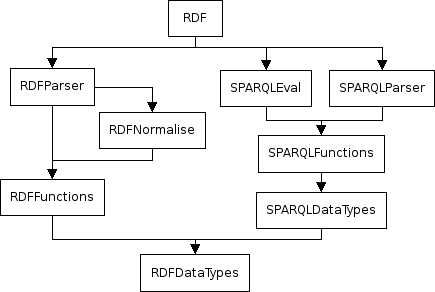
\includegraphics[width=0.85\textwidth]{images/module_hierachie.eps}
\end{figure}   
%------------Chapter Four------------------------
\chapter{Conclusion}\label{concl}
\section{Assessment of the Filter and Arrow Approach}
It has already been mentioned, that the Haskell XML Toolbox has provided a different high-level programming interface than the discussed arrow approach. This interface is still available because of compatibility reasons. The idea of it is to use \textit{filters} for manipulating XML documents. Different combinator functions give the possibility to create complex filters out of simple ones. The data structure used by these filters are the same as the one described above. The generic type \texttt{NTree} defines the tree structure and the specialised type \texttt{XmlTree} with \texttt{XNode} represents the XML document tree. The filter functions have one of the types shown in the next listing:
\begin{code}
type TFilter node = NTree node -> NTrees node
type TSFilter node = NTrees node -> NTrees node
\end{code}
The first one defines a filter which takes a single generic tree and returns a list of trees, while the second filter takes a list of trees and also returns a list of trees. Of course, there are also specialised versions of these types, representing filters for XML trees:
\begin{code}
type XmlFilter = TFilter XNode
type XmlSFilter = TSFilter XNode 
\end{code}
The different filters can be separated in selector-functions, predicates, constructors and functions to manipulate nodes and subtrees, like it has been done with the different arrows. The boolean values \textbf{True} and \textbf{False} are represented by the none-empty list and the empty list, respectively, and there are also filters which embody the identity and the null case. Every function processing the XML document has to be of type \texttt{XmlFilter}, to ensure that they can be combined. One of the often used combinators is the operator \texttt{($>$.)} which represents the sequential composition of filters. It is equivalent to the arrow composition with \texttt{($>$$>$$>$)}.\\
For example, a filter which selects the text of a comment node has the following type:
\begin{code}
getXCmt :: XmlFilter
\end{code}
One would expect, that a filter which selects the text of a comment node would return a character string. But that is not allowed, since the filters all have to be of the same type. The result of the filter \texttt{getXCmt} is therefore encapsulated by a text node stored in a list. If the processed node is not a comment node the resulting list would be empty. The type definition of the arrow providing the same functionality is shown in the next listing:
\begin{code}
getCmt :: a XmlTree String
\end{code}
Comparing the arrow \texttt{getCmt} and the filter \texttt{getXCmt} exhibits the two disadvantages of the filter approach. The first problem is related to the programming style. As every filter function has to be of the same type, the type signature of it does not give any information about the way of operation of the filter. Only the name of the function and a possible description can help to discover what the filter actually does.\\
The second issue with the filter approach is also related to the type. The type checker of the Haskell compiler cannot detect any type errors. Haskell is a strong typed language, which is a big advantage. But by using the same type for all functions, the powerful type system of Haskell is practically switched off. The filter function \texttt{getXCmt} could also return a char reference or a new XML tag instead of the comment-text encapsulated by a text node. As a result, the type checker would not produce an error. This is because \texttt{XmlFilter} is a \textit{type synonym}. There is no way to parameterise this type and to change the input and result type. The programmer has to rely on the description of the filter function, when he wants to process the output of a filter.\\
These problems become irrelevant when using arrows rather then filters. Arrows always have a specified type, the input and output type are specific and not always the same, since the instances of the arrow classes are data types defined with \textit{newtype}. This makes the programming with them much more natural than with filters, since the type system of Haskell is able to react on type errors. Furthermore, the example of the RDF/XML parser has shown, that it is also possible to use other data types for special purposes with the arrows of the Haskell XML Toolbox. The filter approach would not allow this and the data structure of the XML parser has to be used. Everything has to be encapsulated by a \texttt{XmlTree}, although it is senseless.\\
The idea of using filters as the programming interface has been adopted from the XML parser HaXML \cite{HaXML}. The filters of HaXML are all of the following type:
\begin{code}
type CFilter = Content -> [Content]
\end{code}
A filter works for nodes of the type \texttt{Content}. A \texttt{Content} represents the document subset of XML which is only a small part of the whole XML document. In contrast to the data model of the Haskell XML Toolbox, HaXML uses not a generic one but a more data centric approach. The whole XML document is represented by different algebraic data types and almost every production of the XML grammar is modelled with a special type. Therefore, the filters cannot process the whole XML document and if one wants to work with other parts of the document, like the DTD, special functions have to be implemented.\\
The filters of the Haskell XML Toolbox instead give the possibility to process the whole generic data structure, hence the whole document. But nevertheless, HaXML has the same problems with the filter approach as the Haskell XML Toolbox. Type errors cannot be detected by the type system of Haskell. 

\section{Related Work}
There are two other XML parsers written in Haskell, HaXML \cite{HaXML} and HXML \cite{HXML}. HaXML has already been introduced and since it has not an arrow module as the programming interface it will not be taken into consideration in this section. HXML, alternately, has changed its programming interface to arrows recently and will be compared with the Haskell XML Toolbox.\\
HXML is a non-validating parser and does not support XML namespaces but in return it is designed for space-efficiency. Moreover, HXML provides a special adapter to use it as a drop-in replacement for HaXML. The data model used in HXML is quite similar to the one in the Haskell XML Toolbox and has been a pattern for it. The structure of a XML document is modelled by the generic data type \texttt{Tree} and the document subset is represented as a \texttt{Tree} of \texttt{XmlNode}s:
\begin{code}[basicstyle=\ttfamily\small]
type XML     = Tree XMLNode
data Tree a  = Tree a [Tree a]
data XMLNode =
    RTNode                      -- root node
  | ELNode Name [(Name,String)] -- element node: name, attributes
  | TXNode String               -- text node
  | PINode Name String          -- processing instruction (target,value)
  | CXNode String               -- comment node
  | ENNode Name                 -- general entity reference 
\end{code}
DTDs are not stored in the tree model but in a special data type, in contrast to the Haskell XML Toolbox, where the DTD subset is also represented by the generic tree type. Hence, the approach of the Haskell XML Toolbox is much more general. This leads to the fact, that no extra processing functions for DTDs need to be implemented and the functions for processing the XML document subset and the DTD subset are the same.\\
HXML also uses arrows as the high-level programming interface. It follows the same idea as the Haskell XML Toolbox. The processing arrows represent computation over lists. In the Haskell XML Toolbox these arrows are called list arrows and in HXML they are named \textit{filters}:
\begin{code}
newtype Filter a b = Filter (a -> [b])
\end{code} 
The arrow class which is implemented by \texttt{Filter} is provided by HXML and slightly different than the one used by the Haskell XML Toolbox. This is because the idea of arrows has been very new at the moment of the implementation and the compilers GHC or Hugs \cite{HUGS} have not provided this class at that time. Therefore, the arrow class contains several combinators which are not included in the standard arrow class. There are no special combinators for list arrows like they are provided by the class \texttt{ArrowList}. This makes the programming interface of HXML less powerful then the one of the Haskell XML Toolbox. Especially, combinators which solve the problem of the point-free programming are missing. Furthermore, HXML does not provide any state handling. All in all, HXML seems to be in an experimental state in comparison to the Haskell XML Toolbox which offers more functionallity to serve as a professional XML parser.
 
\section{Conclusion and Future Work}
The examples of processing RDF/XML documents have shown that it is straightforward to implement applications with the programming interface of the Haskell XML Toolbox. The resulting RDF/XML parser and the query language extension are very short and compact programs. This is because of the functional language Haskell, which allows to develop in a very problem-oriented way.\\
\\
The new approach of using arrows to process the XML document, has proven to be a flexible and useful way in comparison to the filter approach. Not only XML parsers, but also several other libraries for Haskell and other functional programming languages have adopted this approach recently. The idea of defining ones own notion of computations based on the specific problem provides an attractive programming style. The problem of arrows, using values more than once, i.e. the point-wise programming, can be solved with the arrow notation of Ross Patterson \cite{Pat:2001}. The special operators, provided by the Haskell XML Toolbox, are another way to deal with the problems of the point-free programming.\\
\\
The intention of developing an RDF/XML parser and the SPARQL query language parser was not to design a professional program. Instead, it has demonstrated the way of programming with the Haskell XML Toolbox. Nevertheless, the program parts can be extended easily in order to be used in a professional application, since the arrow interface and the functional approach have made the code understandable and maintainable. The different normalisation steps of RDF/XML can be improved so that they support all abbreviations of the RDF/XML syntax.\\
\\
The Haskell XML Toolbox will be extended and maintained as well. At this moment, a parser for the schema language RelaxNG is written in the context of another master thesis. It also uses the arrow interface of the Haskell XML Toolbox.


\begin{thebibliography}{999}

\bibitem[Bird 1988]{B:1988}
{\it Introduction to Functional Programming using Haskell, second edition},
Richard Bird~(1988),
Prentice Hall Series in Computer Science,
ISBN 0-13-48436-0

\bibitem[CHARMOD]{CHARMOD}
\textit{Character Model for the World Wide Web 1.0}, D\"urst M., Yergeau F., Ishida R., Wolf M., Freytag A., Texin T. (Editors), W3C Working Draft, 20 February 2002. This version is http://www.w3.org/TR/2002/WD-charmod-20020220/. The latest version is http://www.w3.org/TR/charmod/.

\bibitem[DC]{DC}
\textit{Dublin Core Metadata Element Set, Version 1.1: Reference Description}, 02 June 2003. This version is http://dublincore.org/documents/2003/06/02/dces/. The latest version is http://dublincore.org/documents/dces/.

\bibitem[GHC]{GHC}
\textit{The Glasgow Haskell Compiler},
http://www.haskell.org/ghc

\bibitem[HaXML]{HaXML}
{\it HaXML: Haskell and XML}, Mallcom Wallace, http://www.cs.york.ac.uk/fp/HaXml/ .

\bibitem[Hughes 2000]{H:2000}
{\it Generalising monads to arrows},
John Hughes~(2000),
Science of Computer Programming, Volume 37.

\bibitem[Hughes 2004]{H:2004}
{\it Programming with Arrows},
John Hughes~(2004),
In AFP, Tartu, Estonia.

\bibitem [Hugs]{HUGS} 
\textit{Hugs 98}
http://www.haskell.org/hugs/

\bibitem[HXML]{HXML}
{\it HXML}, Joe Englisch, http://www.flightlab.com/~joe/hxml/ .

\bibitem[Jones et al. 1998]{J:1998}
{\it The Haskell 98 Report},
Simon Peyton Jones, John Hughes et al.~(1998),
http://www.haskell.org/onlinereport/ .

\bibitem[N3]{N3}
\textit{Notation 3}, Tim Berners-Lee, http://www.w3.org/DesignIssues/Notation3 .

\bibitem[Parsec]{Parsec}
{\sl Parsec: a free monadic parser combinator library
for Haskell}, Daan Leijen, http://www.cs.uu.nl/$\sim$daan/parsec.html .

\bibitem[Paterson 2001]{Pat:2001}
{\it A new notation for arrows},
Ross Paterson~(2001),
In ICFP, Firenze, Italy. ACM.

\bibitem [Paterson 2003]{Pat:2003}
{\it Arrows and computation},
Ross Paterson~(2003),
In Jeremy Gibbons and Oege De Moor, editors, The Fun of Programming. Palgrave.

\bibitem[RDF Concepts]{RDF:Concepts}
\textit{Resource Description Framework (RDF): Concepts and Abstract Syntax}, Klyne G., Carroll J. (Editors), W3C Recommendation, 10 February 2004. This version is http://www.w3.org/TR/2004/REC-rdf-primer-20040210/. The latest version is http://www.w3.org/TR/rdf-concepts/.

\bibitem[RDF Primer]{RDF:Primer}
\textit{RDF Primer}, Manola F., Miller E., Editors, W3C Recommendation, 10 February 2004. This version is http://www.w3.org/TR/2004/REC-rdf-primer-20040210/. The latest version is at http://www.w3.org/TR/rdf-primer/.

\bibitem[RDF Schema]{RDF:Schema}
\textit{RDF Vocabulary Description Language 1.0: RDF Schema}, Brickley D., Guha R.V. (Editors), W3C Recommendation, 10 February 2004. This version is http://www.w3.org/TR/2004/REC-rdf-schema-20040210/. The latest version  is http://www.w3.org/TR/rdf-schema/.

\bibitem[RDF Sematics]{RDF:Semantics}
\textit{RDF Semantics}, Hayes P. (Editor), W3C Recommendation, 10 February 2004. This version is http://www.w3.org/TR/2004/REC-rdf-mt-20040210/. The latest version is http://www.w3.org/TR/rdf-mt/.

\bibitem[RDF Tests]{RDF:Tests}
\textit{RDF Test Cases}, Grant J., Beckett D. (Editors), W3C Recommendation, 10 February 2004. This version is http://www.w3.org/TR/2004/REC-rdf-testcases-20040210/. The latest version is http://www.w3.org/TR/rdf-testcases/.

\bibitem[RDF/XML Syntax]{RDF:Syntax}
\textit{RDF/XML Syntax Specification (Revised)}, Beckett D. (Editor), W3C Recommendation, 10 February 2004. This version http://www.w3.org/TR/2004/REC-rdf-syntax-grammar-20040210/. The latest version is http://www.w3.org/TR/rdf-syntax-grammar/.

\bibitem[Schmidt 2002]{Schmidt:2002}
{\it Design and Implementation of a validating XML parser in Haskell},
Martin Schmidt~(1999), Master's Thesis .

\bibitem[SPARQL]{SPARQL}
\textit{SPARQL Query Language for RDF}, Prud'hommeaux E., Seaborne A. (Editors), W3C Working Draft, 19 April 2005. This version is http://www.w3.org/TR/2005/WD-rdf-sparql-query-20050419/. The latest version is http://www.w3.org/TR/rdf-sparql-query/.

\bibitem[SPARQL Result]{SPARQL:Result}
\textit{SPARQL Variable Binding Results XML Format}, Beckett D. (Editor), W3C Working Draft, 27 May 2005. This version is http://www.w3.org/TR/2004/WD-rdf-sparql-XMLres-20050527/. The latest version is http://www.w3.org/TR/rdf-sparql-XMLres/.

\bibitem[URIS]{URIS}
\textit{RFC 2396 - Uniform Resource Identifiers (URI): Generic Syntax}, Berners-Lee T., Fielding R., Masinter L., IETF, August 1998, http://www.isi.edu/in-notes/rfc2396.txt.

\bibitem[XML]{XML}
\textit{Extensible Markup Language (XML) 1.0}, Second Edition, Bray T., Paoli J., Sperberg-McQueen C.M., Maler E. (Editors), World Wide Web Consortium, 6 October 2000. This version is http://www.w3.org/TR/2000/REC-xml-20001006. The latest version is http://www.w3.org/TR/REC-xml.

\bibitem[XML-NS]{XML-NS}
\textit{Namespaces in XML}, Bray T., Hollander D., Layman A. (Editors), World Wide Web Consortium, 14 January 1999. This version is http://www.w3.org/TR/1999/REC-xml-names-19990114/. The latest version is http://www.w3.org/TR/REC-xml-names/.

\bibitem[XML Schema]{XML:Schema}
\textit{XML Schema Part 2: Datatypes}, Biron P., Malhotra A. (Editors), World Wide Web Consortium. 2 May 2001. This version is http://www.w3.org/TR/2001/REC-xmlschema-2-20010502/. The latest version is http://www.w3.org/TR/xmlschema-2/.

\end{thebibliography}

\appendix
\chapter{List of Options for \texttt{readDocument} and \texttt{writeDocument}}\label{options}
 \setlongtables 
\begin{longtable}{|l|p{0.689\textwidth}|} \hline
\multicolumn{2}{|c|}{\textbf{Options for readDocument}} \\ \hline
\textbf{Option} & \textbf{Description} \\ \hline
\texttt{a\_parse\_html} & use HTML parser, else use XML parser (default) \\ \hline
\texttt{a\_parse\_html} & use HTML parser, else use XML parser (default)\\ \hline
\texttt{a\_validate} & validate document, else skip validation (default)\\ \hline
\texttt{a\_check\_namespaces} & check namespaces, else skip namespace processing (default)\\ \hline
\texttt{a\_canonicalize} & canonicalise document (default), else skip canonicalisation\\ \hline
\texttt{a\_preserve\_comment} & preserve comments during canonicalisation, else remove comments (default)\\ \hline
\texttt{a\_remove\_whitespace} & remove all whitespace, used for document indentation, else skip this step (default)\\ \hline
\texttt{a\_indent} & indent document by inserting whitespace, else skip this step (default)\\ \hline
\texttt{a\_issue\_warnings} & issue warnings, when parsing HTML (default), else ignore HTML parser warnings\\ \hline
\texttt{a\_issue\_errors} & issue all error messages on stderr (default), or ignore all error messages (default)\\ \hline
\texttt{a\_trace} & trace level: values: 0 - 4\\ \hline
\texttt{a\_proxy} & proxy for http access, e.g. www-cache:3128\\ \hline
\texttt{a\_use\_curl} & for http access via external programm curl, default is native HTTP access\\ \hline
\texttt{a\_options\_curl} & more options for external program curl\\ \hline
\texttt{a\_encoding} & default document encoding (utf8, isoLatin1, usAscii, ...)\\ \hline \hline
\multicolumn{2}{|c|}{\textbf{Options for writeDocument}} \\ \hline 
\texttt{a\_indent} & indent document for readability, (default: no indentation)\\ \hline 
\texttt{a\_remove\_whitespace} & remove all redundant whitespace for shorten text (default: no removal)\\ \hline 
\texttt{a\_output\_encoding} & encoding of document, default is a\_encoding or utf8\\ \hline 
\texttt{a\_output\_xml} & (default) issue XML: quote special XML chars $>$,$<$,",',\& add XML processing instruction and encode document with respect to a\_output\_encoding, if explicitly switched of, the plain text is issued, this is useful for non XML output, e.g. generated Haskell code, LaTex, Java, ...\\ \hline 
\texttt{a\_show\_tree} & show tree representation of document (for debugging)\\ \hline 
\texttt{a\_show\_haskell} & show Haskell representaion of document (for debugging)\\ \hline 
\end{longtable}  

%\chapter{Directory Structure of the enclosed CD}

%\begin{tabular}[c]{l l}
%{\tt $\backslash$ } & the source code of the various modules and the \textit{Makefile} (for usage see below)\\ \\
%{\tt $\backslash$doc$\backslash$} & this document in postscript format and the grammar of the query language\\\\
%{\tt $\backslash$doc$\backslash$hdoc$\backslash$} & the HTML library documentation, generated with Makefile \\ 
%\end{tabular}

%\subsubsection{Usage of Makefile}
%For compiling the sources with GHC:
%\begin{blank}
%    make all
%\end{blank}
%For generating the HTML library documentation:
%\begin{blank}
%    make doc
%\end{blank}

\chapter{Grammar of the Query Language} \label{grammar}
\begin{verbatim}
[1]  Query                          ::= SelectClause WhereClause
[2]  SelectClause                   ::= 'SELECT' Var+ | 'SELECT' '*'
[3]  WhereClause                    ::= 'WHERE' GraphPattern
[4]  GraphPattern                   ::= '{' PatternElementsList '}'
[5]  PatternElementsList            ::= PatternElement PatternElementsListTail ?
[6]  PatternElementsListTail        ::= '.' PatternElementsList ?
[7]  PatternElement                 ::= Triples
                                        | GraphPattern
[8]  Triples                        ::= VarOrTerm PropertyListNotEmpty
[9]  PropertyList                   ::= PropertyListNotEmpty ?
[10] PropertyListNotEmpty           ::= Verb ObjectList PropertyListTail ?
[11] PropertyListTail               ::= ';' PropertyList ?
[12] ObjectList                     ::= Object ObjectTail ?
[13] ObjectTail                     ::= ',' ObjectList ?
[14] Verb                           ::= VarOrURI | 'a'
[15] Object                         ::= VarOrTerm
[16] VarOrURI                       ::= Var | URI
[17] VarOrTerm                      ::= Var | GraphTerm
[18] Var                            ::= <VAR>
[19] GraphTerm                      ::= RDFTerm
[20] RDFTerm                        ::= URI 
                                        | RDFLiteral 
                                        | NumericLiteral
                                        | BooleanLiteral
                                        | BlankNode
[21] NumericLiteral                 ::= Integer | FloatingPoint
[22] RDFLiteral                     ::= String (<LANGTAG> | '^^' URI )?
[23] BooleanLiteral                 ::= 'TRUE' | 'FALSE'
[24] String                         ::= <STRING_LITERAL1> | <STRING_LITERAL2>
[25] URI                            ::= QuotedURIref
[26] BlankNode                      ::= <BNODE_LABEL>
[27] QuotedURIref                   ::= <Q_URIref>
[28] Integer                        ::= <INTEGER_10>
[29] FloatingPoint                  ::= <FLOATING_POINT>
[30] <Q_URIref>                     ::= '<' ([^> ])* '>'  /* RFC 3869 */
[31] <BNODE_LABEL>                  ::= '_:' (<NCNAME2>|<NCNAME1>)
[32] <VAR>                          ::= ('?'|'$') (<NCNAME2>|<NCNAME1>)
[33] <LANGTAG>                      ::= <AT> <A2Z>+ ('-' (<A2ZN>)+)*
[34] <AT>                           ::= '@'
[35] <A2Z>                          ::= [a-zA-Z]
[36] <A2ZN>                         ::= [a-zA-Z0-9]
[37] <INTEGER_10>                   ::= <DIGITS>
[38] <FLOATING_POINT>               ::= [0-9]+ '.' [0-9]* <EXPONENT>? 
                                        | '.' ([0-9])+ <EXPONENT>?
                                        | ([0-9])+ <EXPONENT>
[39] <EXPONENT>                     ::= [eE] [+-]? [0-9]+
[40] <STRING_LITERAL1>              ::= "'" ( ([^'\\\n\r]) | ('\\' [^\n\r]) )* "'"
[41] <STRING_LITERAL2|              ::= '"' ( ([^'\\\n\r]) | ('\\' [^\n\r]) )* '"'
[42] <DIGITS>                       ::= [0-9]+
[43] <NCCHAR1>                      ::= [A-Z]
                                        | [a-z]
                                        | [#x00C0-#x00D6]
                                        | [#x00D8-#x00F6]
                                        | [#x00F8-#x02FF]
                                        | [#x0370-#x037D]
                                        | [#x037F-#x1FFF]
                                        | [#x200C-#x200D]
                                        | [#x2070-#x218F]
                                        | [#x2C00-#x2FEF]
                                        | [#x3001-#xD7FF]
                                        | [#xF900-#xFFFF]
[44] <NCCHAR_END>                   ::= <NCCHAR1> | '_' | '-' | [0-9] | #x00B7
[45] <NCCHAR_FULL>                  ::= <NCCHAR_END> | '.'
[46] <NCNAME1>                      ::= <NCCHAR1> (<NCCHAR_FULL>* <NCCHAR_END>)?
[47] <NCNAME2>                      ::= '_' (<NCCHAR_FULL>* <NCCHAR_END>)?
\end{verbatim}

\chapter{Affidavit}
I hereby declare that this master thesis has been written only by the undersigned and without any assistance from third parties.\\
Furthermore, I confirm that no sources have been used in the preparation of this thesis other than those indicated in the thesis itself.\\
\\
\\
Wedel, \today 
\\
\\

\end{document}


